%%%% Шаблон Отчета по практике <<SPbPU-student-thesis-template>>  %%%%
%%
%%   Создан на основе глубокой переработки шаблона российских кандидатских и докторских диссертаций [1]. 
%%   
%%   Полный список различий может быть получен командами git.
%%   Лист авторов-составителей расположен в README.md файле.
%%   Подробные инструкции по использованию в [1,2].
%%   
%%   Рекомендуем установить TeX Live + TeXstudio
%%   <<Стандартная>> компиляция 2-3 РАЗА с помощью pdflatex + biber (для библиографии)     
%%  
%%%% Student thesis template <<SPbPU-student-thesis-template>> %%%%
%%
%%   Created on the basis of deep modifification of the Russian candidate and doctorate thesis template [1]. 
%%   
%%   Full list of differences can be achieved by git commands.
%%   List of template authors can be seen in the README.md file.
%%   Detailed instructions of usage, see, please in [1,2].
%%     
%%   [1] github.com/AndreyAkinshin/Russian-Phd-LaTeX-Dissertation-Template 
%%   [2] Author_guide_SPBPU-student-thesis-template.pdf
%%   
%%   It is recommended to install TeX Live + TeXstudio   
%%   Default compilation 2-3 TIMES with pdflatex + biber (for the bibliography)
%%  
%%%% Preamble start %%%%  
%%
%%   Please, do not modify files in the preamble
%%
\newcommand*{\anyptfilebase}{template_settings/bpfont} 
\newcommand*{\anyptsize}{14} 		 
\RequirePackage[l2tabu,orthodox]{nag} 
\documentclass[extrafontsizes,a4paper,*pt,oneside,openany]{memoir}
%%%%%%%%%%%%%%%%%%%%%%%%%%%%%%%%%%%%%%%%%%%%%%%%%%%%%%
%%%% Файл упрощённых настроек шаблона диссертации %%%%
%%%%%%%%%%%%%%%%%%%%%%%%%%%%%%%%%%%%%%%%%%%%%%%%%%%%%%

%%% Инициализирование переменных, не трогать!  %%%
\newcounter{intvl}
\newcounter{otstup}
\newcounter{contnumeq}
\newcounter{contnumfig}
\newcounter{contnumtab}
\newcounter{pgnum}
\newcounter{chapstyle}
\newcounter{headingdelim}
\newcounter{headingalign}
\newcounter{headingsize}
\newcounter{tabcap}
\newcounter{tablaba}
\newcounter{tabtita}
\newcounter{docType} 	    % тип документа
\newcounter{tskPrint} 	    % печать Задания на ВКР двух(одно)сторонняя
\newcounter{tskPages}       % для учёта количества страниц в Задании
\newcounter{tskPageFirst}   % для учёта количества страниц в Задании
\newcounter{tskPageLast}    % для учёта количества страниц в Задании 
\newcounter{sumPrint} 	    % печать Реферата на ВКР двух(одно)сторонняя
\newcounter{sumPages}       % для учёта количества страниц в Реферате
\newcounter{sumPageFirst}   % для учёта количества страниц в Реферате
\newcounter{sumPageLast}    % для учёта количества страниц в Реферате 
\newcommand{\Single}{0.78}  % пропорция для одинароного отступа в \Spacing
%%%%%%%%%%%%%%%%%%%%%%%%%%%%%%%%%%%%%%%%%%%%%%%%%%

%%% Область упрощённого управления оформлением %%%

% Управление перенесено в главые файлы компиляции ВКР, Задания, Реферата
\setcounter{tskPrint}{0} %по умолчанию односторонняя печать              
%\setcounter{sumPrint}{0} %по умолчанию односторонняя печать 

%% Интервал между заголовками и между заголовком и текстом
% Заголовки отделяют от текста сверху и снизу тремя интервалами (ГОСТ Р 7.0.11-2011, 5.3.5)
\setcounter{intvl}{3}               % Коэффициент кратности к размеру шрифта

% Заголовки отделяют от текста сверху и снизу тремя интервалами 
\newcommand{\intvlS}{1.5}               % Коэффициент кратности к размеру шрифта SPbPU-student-templates

\newcommand{\intervalS}{\vspace{\intvlS\curtextsize}}

% печать списка источников в Задании
\newcommand{\printbibliographyTask}{\vspace{-0.28\curtextsize}
	\printbibliography[env=tsk] % печать списка литературы в исходных данных
	\vspace{-0.28\curtextsize}}


%% Отступы у заголовков в тексте
\setcounter{otstup}{0}              % 0 --- без отступа; 1 --- абзацный отступ

%% Нумерация формул, таблиц и рисунков
\setcounter{contnumeq}{0}           % Нумерация формул: 0 --- пораздельно (во введении подряд, без номера раздела); 1 --- сквозная нумерация по всей диссертации
\setcounter{contnumfig}{0}          % Нумерация рисунков: 0 --- пораздельно (во введении подряд, без номера раздела); 1 --- сквозная нумерация по всей диссертации
\setcounter{contnumtab}{0}          % Нумерация таблиц: 0 --- пораздельно (во введении подряд, без номера раздела); 1 --- сквозная нумерация по всей диссертации


%% Нумерация подстраничных сносок (ссылок)
%сквозная
\counterwithout{footnote}{chapter} %сквозная нумерация подразделов (во всех главах)


%% Нумерация подразделов
%убрать номер главы в секции
%\counterwithout{section}{chapter} %сквозная нумерация подразделов (во всех главах)
%\renewcommand\thesection{\arabic{section}} %в каждой главе нумерация заново

%\renewcommand\thesection{\arabic{section}}
%\renewcommand\thefigure{\fbox{\arabic{figure}}}
%\renewcommand\thetable{\arabic{table}}
%\renewcommand\theequation{\arabic{equation}}



%\counterwithout{section}{chapter}
%\counterwithout{figure}{chapter}
%\counterwithout{table}{chapter}
%\counterwithout{equation}{chapter}

%\counterwithin{section}{chapter}
%\counterwithin{figure}{chapter}
%\counterwithin{table}{chapter}

%% Оглавление

\setcounter{pgnum}{1}               %NB УДАЛЕНО ФИЗИЧЕСКИ 0 --- номера страниц никак не обозначены; 1 --- Стр. над номерами страниц (дважды компилировать после изменения)  
\settocdepth{subsection} %             до какого уровня подразделов выносить в оглавление
\setsecnumdepth{subsubsection}         % до какого уровня нумеровать подразделы


%% Текст и форматирование заголовков
\setcounter{chapstyle}{1}           % 0 --- разделы только под номером; 1 --- разделы с названием "Глава" перед номером
\setcounter{headingdelim}{2}        % 0 --- номер отделен пропуском в 1em или \quad; 1 --- номера разделов и ений отделены точкой с пробелом, подразделы пропуском без точки; 2 --- номера разделов, подразделов и приложений отделены точкой с пробелом.

%% Выравнивание заголовков в тексте
\setcounter{headingalign}{0}        % 0 --- по центру; 1 --- по левому краю

%% Размеры заголовков в тексте
\setcounter{headingsize}{0}         % 0 --- SPbPU style, все всегда 14 пт; 1 --- пропорционально изменяющийся размер в зависимости от базового шрифта;

%% Подпись таблиц
\setcounter{tabcap}{1}              % 0 --- по ГОСТ, номер таблицы и название разделены тире, выровнены по левому краю, при необходимости на нескольких строках; 1 --- подпись таблицы не по ГОСТ, на двух и более строках, дальнейшие настройки: 
%Выравнивание первой строки, с подписью и номером
\setcounter{tablaba}{2}             % 0 --- по левому краю; 1 --- по центру; 2 --- по правому краю
%Выравнивание строк с самим названием таблицы
\setcounter{tabtita}{1}             % 0 --- по левому краю; 1 --- по центру; 2 --- по правому краю
%Разделитель записи «Таблица #» и названия таблицы
\newcommand{\tablabelsep}{space}   % space = пробел, period =  (определены в подключенных пакетах)

%% Подпись рисунков
%Разделитель записи «Рисунок #» и названия рисунка
\newcommand{\figlabelsep}{period}   % emdash = тире, определён в common/styles; period = точка определён в подключенных пакетах; space
%\newcommand{\figlabelsep}{emdash}   % emdash = тире, определён в common/styles; period = точка определён в подключенных пакетах


%%% Цвета гиперссылок %%%
% Latex color definitions: http://latexcolor.com/

%\definecolor{linkcolor}{rgb}{0.9,0,0}
%\definecolor{citecolor}{rgb}{0,0.6,0}
%\definecolor{urlcolor}{rgb}{0,0,1}


%\definecolor{linkbordercolor}{rgb}{0,0,1}

\definecolor{linkcolor}{HTML}{FF0000} %very light red from the SPbPU brandbook (2nd level)
\definecolor{citecolor}{HTML}{6CF479} %very light green from the SPbPU brandbook (2nd level)
\definecolor{urlcolor}{HTML}{4481BA} %very light blue from the SPbPU brandbook (2nd level)

%\definecolor{linkcolor}{rgb}{0,0,0} %black
%\definecolor{citecolor}{rgb}{0,0,0} %black
%\definecolor{urlcolor}{rgb}{0,0,0} %black               
\input{template_settings/common/packages}  
\input{template_settings/Dissertation/dispackages}         
\input{template_settings/Dissertation/userpackages}         
%%%%%%%%%%%%%%%%%%%%%%%%%%%%%%%%%%%%%%%%%%%%%%%%%%%%%%
%%%% Файл упрощённых настроек шаблона диссертации %%%%
%%%%%%%%%%%%%%%%%%%%%%%%%%%%%%%%%%%%%%%%%%%%%%%%%%%%%%

%%% Инициализирование переменных, не трогать!  %%%
\newcounter{intvl}
\newcounter{otstup}
\newcounter{contnumeq}
\newcounter{contnumfig}
\newcounter{contnumtab}
\newcounter{pgnum}
\newcounter{chapstyle}
\newcounter{headingdelim}
\newcounter{headingalign}
\newcounter{headingsize}
\newcounter{tabcap}
\newcounter{tablaba}
\newcounter{tabtita}
\newcounter{docType} 	    % тип документа
\newcounter{tskPrint} 	    % печать Задания на ВКР двух(одно)сторонняя
\newcounter{tskPages}       % для учёта количества страниц в Задании
\newcounter{tskPageFirst}   % для учёта количества страниц в Задании
\newcounter{tskPageLast}    % для учёта количества страниц в Задании 
\newcounter{sumPrint} 	    % печать Реферата на ВКР двух(одно)сторонняя
\newcounter{sumPages}       % для учёта количества страниц в Реферате
\newcounter{sumPageFirst}   % для учёта количества страниц в Реферате
\newcounter{sumPageLast}    % для учёта количества страниц в Реферате 
\newcommand{\Single}{0.78}  % пропорция для одинароного отступа в \Spacing
%%%%%%%%%%%%%%%%%%%%%%%%%%%%%%%%%%%%%%%%%%%%%%%%%%

%%% Область упрощённого управления оформлением %%%

% Управление перенесено в главые файлы компиляции ВКР, Задания, Реферата
\setcounter{tskPrint}{0} %по умолчанию односторонняя печать              
%\setcounter{sumPrint}{0} %по умолчанию односторонняя печать 

%% Интервал между заголовками и между заголовком и текстом
% Заголовки отделяют от текста сверху и снизу тремя интервалами (ГОСТ Р 7.0.11-2011, 5.3.5)
\setcounter{intvl}{3}               % Коэффициент кратности к размеру шрифта

% Заголовки отделяют от текста сверху и снизу тремя интервалами 
\newcommand{\intvlS}{1.5}               % Коэффициент кратности к размеру шрифта SPbPU-student-templates

\newcommand{\intervalS}{\vspace{\intvlS\curtextsize}}

% печать списка источников в Задании
\newcommand{\printbibliographyTask}{\vspace{-0.28\curtextsize}
	\printbibliography[env=tsk] % печать списка литературы в исходных данных
	\vspace{-0.28\curtextsize}}


%% Отступы у заголовков в тексте
\setcounter{otstup}{0}              % 0 --- без отступа; 1 --- абзацный отступ

%% Нумерация формул, таблиц и рисунков
\setcounter{contnumeq}{0}           % Нумерация формул: 0 --- пораздельно (во введении подряд, без номера раздела); 1 --- сквозная нумерация по всей диссертации
\setcounter{contnumfig}{0}          % Нумерация рисунков: 0 --- пораздельно (во введении подряд, без номера раздела); 1 --- сквозная нумерация по всей диссертации
\setcounter{contnumtab}{0}          % Нумерация таблиц: 0 --- пораздельно (во введении подряд, без номера раздела); 1 --- сквозная нумерация по всей диссертации


%% Нумерация подстраничных сносок (ссылок)
%сквозная
\counterwithout{footnote}{chapter} %сквозная нумерация подразделов (во всех главах)


%% Нумерация подразделов
%убрать номер главы в секции
%\counterwithout{section}{chapter} %сквозная нумерация подразделов (во всех главах)
%\renewcommand\thesection{\arabic{section}} %в каждой главе нумерация заново

%\renewcommand\thesection{\arabic{section}}
%\renewcommand\thefigure{\fbox{\arabic{figure}}}
%\renewcommand\thetable{\arabic{table}}
%\renewcommand\theequation{\arabic{equation}}



%\counterwithout{section}{chapter}
%\counterwithout{figure}{chapter}
%\counterwithout{table}{chapter}
%\counterwithout{equation}{chapter}

%\counterwithin{section}{chapter}
%\counterwithin{figure}{chapter}
%\counterwithin{table}{chapter}

%% Оглавление

\setcounter{pgnum}{1}               %NB УДАЛЕНО ФИЗИЧЕСКИ 0 --- номера страниц никак не обозначены; 1 --- Стр. над номерами страниц (дважды компилировать после изменения)  
\settocdepth{subsection} %             до какого уровня подразделов выносить в оглавление
\setsecnumdepth{subsubsection}         % до какого уровня нумеровать подразделы


%% Текст и форматирование заголовков
\setcounter{chapstyle}{1}           % 0 --- разделы только под номером; 1 --- разделы с названием "Глава" перед номером
\setcounter{headingdelim}{2}        % 0 --- номер отделен пропуском в 1em или \quad; 1 --- номера разделов и ений отделены точкой с пробелом, подразделы пропуском без точки; 2 --- номера разделов, подразделов и приложений отделены точкой с пробелом.

%% Выравнивание заголовков в тексте
\setcounter{headingalign}{0}        % 0 --- по центру; 1 --- по левому краю

%% Размеры заголовков в тексте
\setcounter{headingsize}{0}         % 0 --- SPbPU style, все всегда 14 пт; 1 --- пропорционально изменяющийся размер в зависимости от базового шрифта;

%% Подпись таблиц
\setcounter{tabcap}{1}              % 0 --- по ГОСТ, номер таблицы и название разделены тире, выровнены по левому краю, при необходимости на нескольких строках; 1 --- подпись таблицы не по ГОСТ, на двух и более строках, дальнейшие настройки: 
%Выравнивание первой строки, с подписью и номером
\setcounter{tablaba}{2}             % 0 --- по левому краю; 1 --- по центру; 2 --- по правому краю
%Выравнивание строк с самим названием таблицы
\setcounter{tabtita}{1}             % 0 --- по левому краю; 1 --- по центру; 2 --- по правому краю
%Разделитель записи «Таблица #» и названия таблицы
\newcommand{\tablabelsep}{space}   % space = пробел, period =  (определены в подключенных пакетах)

%% Подпись рисунков
%Разделитель записи «Рисунок #» и названия рисунка
\newcommand{\figlabelsep}{period}   % emdash = тире, определён в common/styles; period = точка определён в подключенных пакетах; space
%\newcommand{\figlabelsep}{emdash}   % emdash = тире, определён в common/styles; period = точка определён в подключенных пакетах


%%% Цвета гиперссылок %%%
% Latex color definitions: http://latexcolor.com/

%\definecolor{linkcolor}{rgb}{0.9,0,0}
%\definecolor{citecolor}{rgb}{0,0.6,0}
%\definecolor{urlcolor}{rgb}{0,0,1}


%\definecolor{linkbordercolor}{rgb}{0,0,1}

\definecolor{linkcolor}{HTML}{FF0000} %very light red from the SPbPU brandbook (2nd level)
\definecolor{citecolor}{HTML}{6CF479} %very light green from the SPbPU brandbook (2nd level)
\definecolor{urlcolor}{HTML}{4481BA} %very light blue from the SPbPU brandbook (2nd level)

%\definecolor{linkcolor}{rgb}{0,0,0} %black
%\definecolor{citecolor}{rgb}{0,0,0} %black
%\definecolor{urlcolor}{rgb}{0,0,0} %black               
\input{template_settings/Dissertation/preamblenames}       
\input{template_settings/common/styles}    
%%% Изображения %%%
\graphicspath{{images/}{Dissertation/images/}}         % Пути к изображениям

%%% Макет страницы %%%
% Выставляем значения полей (ГОСТ 7.0.11-2011, 5.3.7)
\makeatletter
\geometry{a4paper,top=2cm,bottom=2cm,left=3cm,right=1cm,
	headsep=0.5cm, %отступ от колонтитула от живописного поля
	head=1cm, %верхняя граница колонтитула
	headheight=1cm,
	nofoot,
%includefoot,
	nomarginpar
%	,showframe
} 
%\setlength{\topskip}{0pt}   %размер дополнительного верхнего поля
\makeatother

%%% Интервалы %%%
%% По ГОСТ Р 7.0.11-2011, пункту 5.3.6 требуется полуторный интервал
%% Реализация средствами класса (на основе setspace) ближе к типографской классике.
%% И правит сразу и в таблицах (если со звёздочкой) 
%\DoubleSpacing*     % Двойной интервал
\OnehalfSpacing*    % Полуторный интервал % * to force it in the floats
%\setSpacing{1.42}   % Полуторный интервал, подобный Ворду (возможно, стоит включать вместе с предыдущей строкой)

%https://tex.stackexchange.com/questions/65849/confusion-onehalfspacing-vs-spacing-vs-word-vs-the-world/276516#276516
%https://tex.stackexchange.com/questions/13742/what-does-double-spacing-mean
%https://tex.stackexchange.com/questions/30073/why-is-the-linespread-factor-as-it-is/30114#30114

%A possible definition of \onehalfspacing and \doublespacing is that the ratio between font size and \baselineskip should be 1.5 resp. 2.....
%\baselineskip (vertical skip between the base lines of two successive lines of type) of XXpt. 


%%% Выравнивание и переносы %%%
%% http://tex.stackexchange.com/questions/241343/what-is-the-meaning-of-fussy-sloppy-emergencystretch-tolerance-hbadness
%% http://www.latex-community.org/forum/viewtopic.php?p=70342#p70342
\tolerance 1414
\hbadness 1414
\emergencystretch 1.5em % В случае проблем регулировать в первую очередь
\hfuzz 0.3pt
\vfuzz \hfuzz
%\raggedbottom
%\sloppy                 % Избавляемся от переполнений
\clubpenalty=10000      % Запрещаем разрыв страницы после первой строки абзаца
\widowpenalty=10000     % Запрещаем разрыв страницы после последней строки абзаца

%%% Блок управления параметрами для выравнивания заголовков в тексте %%%
\newlength{\otstuplen}
\setlength{\otstuplen}{\theotstup\parindent}
\ifnumequal{\value{headingalign}}{0}{% выравнивание заголовков в тексте
    \newcommand{\hdngalign}{\centering}                % по центру
    \newcommand{\hdngaligni}{}% по центру
    \setlength{\otstuplen}{0pt}
}{%
    \newcommand{\hdngalign}{}                 % по левому краю
    \newcommand{\hdngaligni}{\hspace{\otstuplen}}      % по левому краю
} % В обоих случаях вроде бы без переноса, как и надо (ГОСТ Р 7.0.11-2011, 5.3.5)







%%% Оглавление %%%

\renewcommand{\cftchapterdotsep}{\cftdotsep}                % отбивка точками до номера страницы начала главы/раздела



%% снятие жирности %%
%\cftKleader defines the leader between the title and the page number; it can be
%changed by \renewcommand. The spacing between any dots in the leader is controlled
%by \cftKdotsep
\makeatletter
\renewcommand{\cftchapterpagefont}{\normalfont}        % нежирные номера страниц у глав в оглавлении
\renewcommand{\cftchapterleader}{\cftdotfill{\cftchapterdotsep}}% нежирные точки до номеров страниц у глав в оглавлении
\renewcommand{\cftchapterfont}{}                       % нежирные названия глав в оглавлении
\renewcommand{\cftchapterpagefont}{}                       % нежирные названия номеров глав в оглавлении
\makeatother


%% Форматирование SPbPU %%
% Варианты форматирования
%https://tex.stackexchange.com/questions/394227/memoir-toc-indent-the-second-line-by-numberspace-width-in-the-previous-line-or



%% работа с расстояниями между точками, переносами слов
\makeatletter
\renewcommand{\cftdotsep}{0.1}
%\renewcommand{\@dotset}{0.1} %old macro DOES NOT WORK
\setpnumwidth{2.84538em} %2.84538em = 1cm  
%\renewcommand{\@pnumwidth}{0em} %old macro
%%\setrmarg > \setpnumwidth !!!
\setrmarg{2.84539em}
%set large number to restrict hyphenation
%plus1fil makes the distance between the words smaller!
%it helps to make the equal indent
\makeatother

%\usepackage{tocloft}    % tocloft for table of contents style

%% отступы %%
\makeatletter
\renewcommand{\cftchapterbreak}{}        % set a page break before rather than after the entry
%\renewcommand{\cftparskip}{10em} % эта настройка не работает, вместо неё изменен \parskip непостредственно перед \tableofcontents
\setlength{\cftbeforechapterskip}{0pt plus 0pt} %delete skip after chapter block (last section) %%%<-SPbPU pure
\setlength{\cftbeforepartskip}{0pt plus 0pt} %delete skip after chapter block (last section) %%%<-SPbPU pure
\makeatother



%% Продолжение редактирования оглавления настройками CandDoctDiss %%		


\ifnumgreater{\value{headingdelim}}{0}{%
	%<- SPbPU точка после номера страницы
	\renewcommand\cftchapteraftersnum{.\space}       % добавляет точку с пробелом после номера раздела в оглавлении
	%\renewcommand\cftchapteraftersnumb{\enspace\textperiodcentered\enspace} %\enspace - настоящий пробел, \space не работает
	%\renewcommand\chapternumberlinebox[2]{#2}
}{}
\ifnumgreater{\value{headingdelim}}{1}{%%%<-SPbPU 
	%	   	\renewcommand\cftsectionpresnum{..}       % добавляет smth перед number %выравнивает в box
	% точка после номера страницы
	\renewcommand\cftsectionaftersnum{.\space}       % добавляет точку с пробелом после номера подраздела в оглавлении
	% last is \hfil !
	%   	\renewcommand\cftsectionaftersnumb{...}       % добавляет точки перед названием %можно удалить пробел
	\renewcommand\cftsubsectionaftersnum{.\space}    % добавляет точку с пробелом после номера подподраздела в оглавлении
	\renewcommand\cftsubsubsectionaftersnum{.\space} % добавляет точку с пробелом после номера подподподраздела в оглавлении
	\AtBeginDocument{% без этого polyglossia сама всё переопределяет
		\setsecnumformat{\csname the#1\endcsname.\space}
		%\setsecnumformat{\csname the#1\endcsname:\quad}
	}
}{%
	\AtBeginDocument{% без этого polyglossia сама всё переопределяет
		\setsecnumformat{\csname the#1\endcsname\quad} %
	}
}

\renewcommand*{\cftappendixname}{\appendixname\space} % Слово Приложение в оглавлении


%%% Различные варианты форматирования SPbPU %%%

%% форматирование отсупов до номеров страниц стр. 151 мемуара !!!
%\renewcommand*{\cftsectionnumwidth}{} %выставление абсолютного значения
%\addtolength{\cftsectionnumwidth}{5em} %не работает

%убираем фиксированные размеры of the box %%%<-SPbPU pure
\AtBeginDocument{%
\renewcommand\numberlinebox[2]{#2} % for sections %%%<-SPbPU pure
\renewcommand\chapternumberlinebox[2]{#2} % for chapters 
%\newcommand\chapternumberlinebox[2]{%
%	\hb@xt@#1{#2\hfil}}
%
%\newcommand\chapternumberlinebox[2]{%
%	#1{\hfil#2}}

%\numberlinebox{hlengthi}{hcodei} %выставление абсолютного значения
%\chapternumberlinebox{hlengthi}{hcodei} %выставление абсолютного значения
}

%убираем растояния до \cftsectionpresnum в размере одного абзацного отступа %%%<-SPbPU pure
%\cftsetindents{hkindi}{hindenti}{hnumwidthi}


%https://tex.stackexchange.com/questions/306851/multiline-unnumbered-chapter-in-table-of-contents
%https://tex.stackexchange.com/questions/40022/customized-table-of-contents-same-indentation-for-every-line-of-multi-line-titl
%\parindent % standart padding
% это здорово экономит место, но нужно тогда синхронизировать стиль обычных отступов в перечислениях
% недостаток - не видно выравнивания по первому слову в названии предыдущего раздела
\AtBeginDocument{
	\cftsetindents{chapter}{0pt}{% первая строка
		-0.05em} % последующие строки от первой
	\cftsetindents{section}{%
		0pt
%3.5ex plus 1ex minus .2ex
	}{%
		\parindent
%2.3ex plus .2ex
}
	\cftsetindents{subsection}{%
	0pt}{% 
		\parindent}
	\cftsetindents{subsubsection}{%
		0pt}{% 
		\parindent}
}



%%% Колонтитулы %%%
% Порядковый номер страницы печатают на середине верхнего поля страницы (ГОСТ Р 7.0.11-2011, 5.3.8)
%сделаем справа внизу
%\makeatletter
\makeevenhead{plain}{}{}{\thepage}
\makeoddhead{plain}{}{}{\thepage}
\makeevenfoot{plain}{}{}{}
\makeoddfoot{plain}{}{}{}
\pagestyle{plain}

%%% добавить Стр. над номерами страниц в оглавлении
%%% http://tex.stackexchange.com/a/306950
\newif\ifendTOC
%
\newcommand*{\tocheader}{
%\ifnumequal{\value{pgnum}}{1}{%
%    \ifendTOC\else\hbox to \linewidth%
%      {\noindent{}~\hfill{Pages}}\par%
%      \ifnumless{\value{page}}{3}{}{%
%        \vspace{0.5\onelineskip}
%      }
%      \afterpage{\tocheader}
%    \fi%
%}{}%
}%


%epigraph with DOI
%\usepackage{quotchap}




%%% SPbPU %%% Оформление заголовков глав, разделов, подразделов %%%

\newcommand{\printTheAbstract}{%распечатать the Abstract
	\begingroup
	\par
	\renewcommand{\cleardoublepage}{}
	\renewcommand{\clearpage}{}
	\vspace{\theintvl\curtextsize}
	\chapter*{Abstract}
	\endgroup %after chapter in case of inline using
	\thispagestyle{empty}%
}


\makechapterstyle{SPbPUstyle}{%
	\chapterstyle{default}
	\setlength{\beforechapskip}{0pt}
	\setlength{\midchapskip}{0pt} 
	\setlength{\afterchapskip}{\intvlS\curtextsize}
	\renewcommand*{\chapnamefont}{\normalfont\bfseries\MakeTextUppercase} %не используется слово <<Глава>>
	\renewcommand*{\chapnumfont}{\normalfont\bfseries\MakeTextUppercase}
%	\renewcommand*{\chaptitlefont}{\normalfont\bfseries\MakeTextUppercase} %не работает \MakeTextUppercase
	\renewcommand\printchaptertitle{\normalfont\bfseries\MakeTextUppercase}% аналог \chaptitlefont
	\renewcommand*{\chapterheadstart}{}
	\ifnumgreater{\value{headingdelim}}{0}{%
		\renewcommand*{\afterchapternum}{.\space}   % добавляет точку с пробелом после номера раздела
	}{%
		\renewcommand*{\afterchapternum}{.\quad}     % добавляет точку и \space (\quad) после номера раздела
	} % настройки добавление в СОДЕРЖАНИЕ (по умолчанию название раздела переходит само)
	\renewcommand*{\printchapternum}{\hdngaligni\hdngalign\chapnumfont \thechapter}
	\renewcommand*{\printchaptername}{}
	\renewcommand*{\printchapternonum}{\hdngaligni\hdngalign}
	}
\newcommand{\chapterLight}{\normalfont\MakeTextUppercase\normalsize} %не менять последовательность команд!
\renewcommand*{\printtoctitle}[1]{\normalfont\MakeTextUppercase #1} %слово <<Content>> в стилю chaperLight, по факту убираем \bfseries
%\chapterLight не действует в этой команде
\makeatletter


\makechapterstyle{SPbPUstylechapname}{% для <<будет вписано слово Глава перед каждым номером раздела в оглавлении>>
	\chapterstyle{SPbPUstyle}
	\renewcommand*{\printchapternum}{\chapnumfont \thechapter}
	\renewcommand*{\printchaptername}{\hdngaligni\hdngalign\chapnamefont \@chapapp} %

}
\makeatother

\chapterstyle{SPbPUstyle}

%% удалить перенос на новую строку перед командой \chapter
\newcommand{\delnewpagebeforech}{
	%\begingroup
	\renewcommand{\cleardoublepage}{}
	\renewcommand{\clearpage}{}
	\vspace{\theintvl\curtextsize}
	%\endgroup %after chapter in case of inline using
}

%% Оформление шрифтов и отсупов подразделов, подподразделов и подподподразделов

\makeatletter
\setsecheadstyle{\normalfont\bfseries\hdngalign}
\setsecindent{\otstuplen} %отступ от левого края живописного поля
\setbeforesecskip{\intvlS\curtextsize} %базовые настройки с плюс/минус точностью, что позволяет более гибко располагать рисунки и изображения на странице
\setaftersecskip{\intvlS\curtextsize}


\setsubsecheadstyle{\normalfont\bfseries\itshape\hdngalign}
\setsubsecindent{\otstuplen}
\setbeforesubsecskip{1\curtextsize}
\setaftersubsecskip{1\curtextsize}

\setsubsubsecheadstyle{\normalfont\itshape\hdngalign}
\setsubsubsecindent{\otstuplen}
\setbeforesubsubsecskip{1\curtextsize}
\setaftersubsubsecskip{1\curtextsize}

%ОLD  ГИА
%\setsubsecheadstyle{\normalfont\hdngalign}
%\setsubsecindent{\otstuplen}
%\setbeforesubsecskip{\intvlS\curtextsize}
%\setaftersubsecskip{\intvlS\curtextsize}
%
%\setsubsubsecheadstyle{\normalfont\hdngalign}
%\setsubsubsecindent{\otstuplen}
%\setbeforesubsubsecskip{\intvlS\curtextsize}
%\setaftersubsubsecskip{\intvlS\curtextsize}
\makeatother

%попытки форматирования \part можно продолжить
%сейчас реализован более простой вариант
\renewcommand{\partnamefont}{\LARGE\MakeTextUppercase}
\renewcommand{\partnumfont}{\LARGE\MakeTextUppercase}
\renewcommand*{\parttitlefont}{\LARGE\MakeTextUppercase}

%[section], чтобы заставить все floats быть до расположиться до окончания подраздела
%\FloatBarrier локальное ограничение, чтобы 
% расставить повсеместно по разделам, то всего лишь подключить [section];
% разрешить до \FloatBarrier размещать foats, то добавить окцию  [above].
\usepackage[above]{placeins} 

\sethangfrom{\noindent #1} %все заголовки подразделов центрируются с учетом номера, как block 

\ifnumequal{\value{chapstyle}}{1}{%
    \chapterstyle{SPbPUstylechapname}
    \renewcommand*{\cftchaptername}{Глава\space} % будет вписано слово Глава перед каждым номером раздела в оглавлении
}{}% вместо Chapter \chaptername

%%% Интервалы между заголовками
%\setbeforesecskip{\theintvl\curtextsize}% Заголовки отделяют от текста сверху и снизу тремя интервалами (ГОСТ Р 7.0.11-2011, 5.3.5).
%\setaftersecskip{\theintvl\curtextsize}
%\setbeforesubsecskip{\theintvl\curtextsize}
%\setaftersubsecskip{\theintvl\curtextsize}
%\setbeforesubsubsecskip{\theintvl\curtextsize}
%\setaftersubsubsecskip{\theintvl\curtextsize}


%%% Блок дополнительного управления размерами заголовков
\ifnumequal{\value{headingsize}}{1}{% Пропорциональные заголовки и базовый шрифт 14 пт
	\renewcommand{\normalfont}{\large\bfseries}
	\renewcommand*{\chapnamefont}{\Large\bfseries}
	\renewcommand*{\chapnumfont}{\Large\bfseries}
	\renewcommand*{\chaptitlefont}{\Large\bfseries}
}{}




% ОФОРМЛЕНИЕ Приложений Appendix - Вариант 2 - действующий
%https://stackoverflow.com/questions/717316/how-to-make-appendix-appear-in-toc-in-latex
\makeatletter
\newcommand\appendix@chapter[1]{%
	\renewcommand*{\chapnamefont}{\normalfont\normalsize\bfseries} %не используется слово <<Глава>>
	\renewcommand*{\chapnumfont}{\normalfont\normalsize\bfseries}
	\renewcommand\printchaptertitle{\normalfont\normalsize\bfseries}
	\renewcommand*{\printchapternum}{\chapnumfont \thechapter}
	\renewcommand*{\printchaptername}{\hdngaligni\hdngalign\chapnamefont \@chapapp} %
	\renewcommand*\thechapter{\arabic{chapter}} % работает
	\settocdepth{chapter} % выводить только названия Приложений
	\refstepcounter{chapter}%
	\def\app@ct{\hfill{}\appendixname{} {}\@arabic\c@chapter %
%	\vspace{\intvlS\curtextsize}
	\newline #1
	\vspace{\curtextsize}
}
	\orig@chapter*{\app@ct}%
	\addcontentsline{toc}{chapter}{\appendixname{} \@arabic\c@chapter. #1}%\app@ct % input to TOC-table
}
\let\orig@chapter\chapter
\g@addto@macro\appendix{\newpage\let\chapter\appendix@chapter\renewcommand*{\afterchapternum}{\par\nobreak\vskip \midchapskip}}
\makeatother


%https://tex.stackexchange.com/questions/250834/dont-break-page-for-new-chapter-unless-chapter-heading-wont-fully-fit-on-curre
\newcommand{\ContinueChapterBegin}{%
\let\clearpage\relax
\renewcommand*{\chapterheadstart}{%
	\FloatBarrier % make floats stop
\par
\ifartopt % если сверху сраницы, то
% ничего не делать
\else % в противном случае
\vspace{\theintvl\curtextsize} % добавить интервал
\fi
}
}%

\newcommand{\ContinueChapterEnd}{%
	\let\clearpage\newpage
\renewcommand*{\chapterheadstart}{% ничего не делаем
\FloatBarrier % make floats stop
}
}%

\newcommand{\NewPage}{% в случае, если на последней странице приложения есть <<висячая>> таблица или рисунок
\newpage\leavevmode\thispagestyle{plain}\newpage %начать новое приложение с новой страницы 
}%




\makeatletter %настройка отображения floates
\setlength{\@fptop}{0pt}%отключить вертикальное центрирование рисунка/таблицы на странице
%\setlength{\@fpsep}{8pt}%отключить вертикальное центрирование рисунка/таблицы на странице
%\setlength{\@fpbot}{0pt plus 1fil}%отключить вертикальное центрирование рисунка на странице
\makeatother



%%% Счётчики %%%

%% DOI
\newcounter{mychapternumber} 
\newcounter{chapterDOI}

%% Упрощённые настройки шаблона диссертации: нумерация формул, таблиц, рисунков
\ifnumequal{\value{contnumeq}}{1}{%
    \counterwithout{equation}{chapter} % Убираем связанность номера формулы с номером главы/раздела
}{}
\ifnumequal{\value{contnumfig}}{1}{%
    \counterwithout{figure}{chapter}   % Убираем связанность номера рисунка с номером главы/раздела
}{}
\ifnumequal{\value{contnumtab}}{1}{%
    \counterwithout{table}{chapter}    % Убираем связанность номера таблицы с номером главы/раздела
}{}


%%%http://www.linux.org.ru/forum/general/6993203#comment-6994589 (используется totcount)
\makeatletter
\def\formbytotal#1#2#3#4#5{%
    \newcount\@c
    \@c\totvalue{#1}\relax
    \newcount\@last
    \newcount\@pnul
    \@last\@c\relax
    \divide\@last 10
    \@pnul\@last\relax
    \divide\@pnul 10
    \multiply\@pnul-10
    \advance\@pnul\@last
    \multiply\@last-10
    \advance\@last\@c
    \total{#1}~#2%
    \ifnum\@pnul=1#5\else%
    \ifcase\@last#5\or#3\or#4\or#4\or#4\else#5\fi
    \fi
}
\makeatother

% xassoccnt to make total values: tables, figures, chapters 
%https://tex.stackexchange.com/questions/295857/calculate-amount-of-figures?noredirect=1
\NewTotalDocumentCounter{mytotalfigures}
\NewTotalDocumentCounter{mytotalfiguresInApp}
\NewTotalDocumentCounter{mytotaltables}
\NewTotalDocumentCounter{mytotaltablesInApp}
\NewTotalDocumentCounter{myappendices}
\DeclareAssociatedCounters{figure}{mytotalfigures}
\DeclareAssociatedCounters{table}{mytotaltables}

%https://tex.stackexchange.com/questions/317434/mytotal-pages-number-warning-and-miscalculated
%\NewTotalDocumentCounter{mytotalpages} % not supported yet in xassoccnt, use totpages package
%\DeclareAssociatedCounters{page}{mytotalpages}

%счетчики для вывода на печать
\newcounter{mypages} % счетчик 
\setcounter{mypages}{0} % 
\newcounter{mytotalpagesInApp} % cчетчик 
\setcounter{mytotalpagesInApp}{0} %
\newcounter{myfigures} % счетчик 
\setcounter{myfigures}{0} % 
\newcounter{mytables} % счетчик 
\setcounter{mytables}{0} %  




\AtBeginDocument{
	%% регистрируем счётчики в системе totcounter
	%% позволяет использовать: 
	%% 1) команду \total{counter} для печати значения
	%% 2) спрягать значения слов с помощью \formbytotal
	\regtotcounter{mypages}      % simple counter
	\regtotcounter{TotPages}     % totpages package
	\regtotcounter{myfigures}      % simple counter
	\regtotcounter{mytotalfigures} % xassoccnt package
	\regtotcounter{mytables}      % simple counter
	\regtotcounter{mytotaltables} % xassoccnt package
	\regtotcounter{myappendices}  % xassoccnt package
}
\newtotcounter{citenum} %счетчик для библиографии из totcount package


\preto\appendix{% когда будет команда \appendix 
	% см. также выше переопределение chapter для appendix
	%% Сохранение сумм: рисунки, таблицы, страницы.
	\setcounter{mytotalpagesInApp}{\value{TotPages}}% 
	% count total values
	\AddAssociatedCounters{figure}{mytotalfiguresInApp}
	\AddAssociatedCounters{table}{mytotaltablesInApp}
	\AddAssociatedCounters{chapter}{myappendices}
	%% Форматирование
	%\renewcommand\thechapter{\arabic{chapter}} % см. переопределение chapter для appendix
	\renewcommand{\appendixname}{Приложение} %
	\renewcommand{\thetable}{П\thechapter.\arabic{table}}
	\renewcommand{\thefigure}{П\thechapter.\arabic{figure}}
	\renewcommand{\theequation}{П\thechapter.\arabic{equation}}
	\renewcommand{\thesection}{П\thechapter.\arabic{section}}
	\renewcommand{\thesubsection}{\thesection.\arabic{subsection}}
	\renewcommand{\thesubsubsection}{\thesubsection.\arabic{subsubsection}}
	\counterwithin{footnote}{chapter} %связанная нумерация глав-сносок
	\renewcommand{\thefootnote}{П\thechapter.\arabic{footnote}}
}


%%% Подсчет сумм: рисунки, таблицы, страницы
%% Вариант 1 (рабочий)
\AtEndDocument{
	\setcounter{myfigures}{\value{mytotalfigures}}%
	\addtocounter{myfigures}{-\value{mytotalfiguresInApp}}%
	\setcounter{mytables}{\value{mytotaltables}}%
	\addtocounter{mytables}{-\value{mytotaltablesInApp}}%
	\setcounter{mypages}{\value{mytotalpagesInApp}}%
	\addtocounter{mypages}{1}%
%	\addtocounter{mypages}{-\value{mytotalpagesInApp}}%
}
%% Вариант 2 (для отладки)
%% работает только в месте вывода на экран суммы, т.е. в реферате
%\setcounter{myfigures}{\numexpr\TotalValue{mytotalfigures}-\TotalValue{mytotalfiguresInApp}\relax}



%%% Правильная нумерация приложений %%%
%% По ГОСТ 2.105, п. 4.3.8 Приложения обозначают заглавными буквами русского алфавита,
%% начиная с А, за исключением букв Ё, З, Й, О, Ч, Ь, Ы, Ъ.
%% Здесь также переделаны все нумерации русскими буквами.
%\ifxetexorluatex
%    \makeatletter
%    \def\russian@Alph#1{\ifcase#1\or
%       А\or Б\or В\or Г\or Д\or Е\or Ж\or
%       И\or К\or Л\or М\or Н\or
%       П\or Р\or С\or Т\or У\or Ф\or Х\or
%       Ц\or Ш\or Щ\or Э\or Ю\or Я\else\xpg@ill@value{#1}{russian@Alph}\fi}
%    \def\russian@alph#1{\ifcase#1\or
%       а\or б\or в\or г\or д\or е\or ж\or
%       и\or к\or л\or м\or н\or
%       п\or р\or с\or т\or у\or ф\or х\or
%       ц\or ш\or щ\or э\or ю\or я\else\xpg@ill@value{#1}{russian@alph}\fi}
%    \makeatother
%\else
%    \makeatletter
%    \if@uni@ode
%      \def\russian@Alph#1{\ifcase#1\or
%        А\or Б\or В\or Г\or Д\or Е\or Ж\or
%        И\or К\or Л\or М\or Н\or
%        П\or Р\or С\or Т\or У\or Ф\or Х\or
%        Ц\or Ш\or Щ\or Э\or Ю\or Я\else\@ctrerr\fi}
%    \else
%      \def\russian@Alph#1{\ifcase#1\or
%        \CYRA\or\CYRB\or\CYRV\or\CYRG\or\CYRD\or\CYRE\or\CYRZH\or
%        \CYRI\or\CYRK\or\CYRL\or\CYRM\or\CYRN\or
%        \CYRP\or\CYRR\or\CYRS\or\CYRT\or\CYRU\or\CYRF\or\CYRH\or
%        \CYRC\or\CYRSH\or\CYRSHCH\or\CYREREV\or\CYRYU\or
%        \CYRYA\else\@ctrerr\fi}
%    \fi
%    \if@uni@ode
%      \def\russian@alph#1{\ifcase#1\or
%        а\or б\or в\or г\or д\or е\or ж\or
%        и\or к\or л\or м\or н\or
%        п\or р\or с\or т\or у\or ф\or х\or
%        ц\or ш\or щ\or э\or ю\or я\else\@ctrerr\fi}
%    \else
%      \def\russian@alph#1{\ifcase#1\or
%        \cyra\or\cyrb\or\cyrv\or\cyrg\or\cyrd\or\cyre\or\cyrzh\or
%        \cyri\or\cyrk\or\cyrl\or\cyrm\or\cyrn\or
%        \cyrp\or\cyrr\or\cyrs\or\cyrt\or\cyru\or\cyrf\or\cyrh\or
%        \cyrc\or\cyrsh\or\cyrshch\or\cyrerev\or\cyryu\or
%        \cyrya\else\@ctrerr\fi}
%    \fi
%    \makeatother
%\fi


%%% Алгоритмы %%%

%\usepackage[linesnumbered]{algorithm2e}
\usepackage[linesnumbered,vlined,figure,scleft]{algorithm2e}

%% Glogal params %%
%ruled, tworuled, algoruled --- put lines to wrap the caption plus a line at the bottom (top) - one should not use this together with inline captions!
%vlined 										--- instead of begin...end will be lines
%boxed 											--- make a box
% figure 										--- count as Fig. ...


% Settings of caption       --- if one will use \caption{} option 	instead of inline + environment caption.
%\SetAlgoCaptionSeparator{.}
%\SetAlgorithmName{Algorithm}{} %last arg is the title of listing table


% Settings for lines numbers
\SetNlSkip{0em}							% sets the value of the space between the line numbers and the text, by default 1em.
\SetNlSty{normalsize}{\hphantom{0}}{.}%defines how to print line numbers
%\hspace*{5mm} does not work 
\SetAlgoNlRelativeSize{-1}	% sets the relative size of line numbers. By default, line numbers are two size smaller than algorithm text

% How to ignore line nuber and to wrap
%http://tex.stackexchange.com/questions/153646/algorithm2e-disabling-line-numbers-for-specific-lines
%http://tex.stackexchange.com/questions/86580/how-to-adjust-line-numbers-of-algorithm2e-package
\makeatletter
%\newcommand{\nosemic}{\renewcommand{\@endalgocfline}{\relax}}% Drop semi-colon ;
%\newcommand{\dosemic}{\renewcommand{\@endalgocfline}{\algocf@endline}}% Reinstate semi-colon ;
%\newcommand{\pushline}{\Indp}% Indent
%\newcommand{\popline}{\Indm\dosemic}% Undent
\let\oldnl\nl% Store \nl in \oldnl
\newcommand{\nonl}{\renewcommand{\nl}{\let\nl\oldnl}}% Remove line number for one line
\makeatother


% Settings for vlines 			
%\SetInd{0.3em}{0.5em}			%default and spaces before and after are 0.5em and 1em
%\SetVlineSkip{5em}					% Sets the value of the vertical space after the little horizontal line which closes a block in vlined mode

%% User abbreviations for ASTRA %%
\SetKwInput{KwInput}{Input}
\SetKwInput{KwOutput}{Output}
%% See also %%
%http://tex.stackexchange.com/questions/145114/caption-below-boxed-algorithm2e-when-used-as-a-figure
%http://tex.stackexchange.com/questions/83536/align-comments-in-algorithm-with-package-algorithm2e



           
% для вертикального центрирования ячеек в tabulary
\def\zz{\ifx\[$\else\aftergroup\zzz\fi}
%$ \] % <-- чиним подсветку синтаксиса в некоторых редакторах
\def\zzz{\setbox0\lastbox
\dimen0\dimexpr\extrarowheight + \ht0-\dp0\relax
\setbox0\hbox{\raise-.5\dimen0\box0}%
\ht0=\dimexpr\ht0+\extrarowheight\relax
\dp0=\dimexpr\dp0+\extrarowheight\relax 
\box0
}



\lstdefinelanguage{Renhanced}%
{keywords={abbreviate,abline,abs,acos,acosh,action,add1,add,%
        aggregate,alias,Alias,alist,all,anova,any,aov,aperm,append,apply,%
        approx,approxfun,apropos,Arg,args,array,arrows,as,asin,asinh,%
        atan,atan2,atanh,attach,attr,attributes,autoload,autoloader,ave,%
        axis,backsolve,barplot,basename,besselI,besselJ,besselK,besselY,%
        beta,binomial,body,box,boxplot,break,browser,bug,builtins,bxp,by,%
        c,C,call,Call,case,cat,category,cbind,ceiling,character,char,%
        charmatch,check,chol,chol2inv,choose,chull,class,close,cm,codes,%
        coef,coefficients,co,col,colnames,colors,colours,commandArgs,%
        comment,complete,complex,conflicts,Conj,contents,contour,%
        contrasts,contr,control,helmert,contrib,convolve,cooks,coords,%
        distance,coplot,cor,cos,cosh,count,fields,cov,covratio,wt,CRAN,%
        create,crossprod,cummax,cummin,cumprod,cumsum,curve,cut,cycle,D,%
        data,dataentry,date,dbeta,dbinom,dcauchy,dchisq,de,debug,%
        debugger,Defunct,default,delay,delete,deltat,demo,de,density,%
        deparse,dependencies,Deprecated,deriv,description,detach,%
        dev2bitmap,dev,cur,deviance,off,prev,,dexp,df,dfbetas,dffits,%
        dgamma,dgeom,dget,dhyper,diag,diff,digamma,dim,dimnames,dir,%
        dirname,dlnorm,dlogis,dnbinom,dnchisq,dnorm,do,dotplot,double,%
        download,dpois,dput,drop,drop1,dsignrank,dt,dummy,dump,dunif,%
        duplicated,dweibull,dwilcox,dyn,edit,eff,effects,eigen,else,%
        emacs,end,environment,env,erase,eval,equal,evalq,example,exists,%
        exit,exp,expand,expression,External,extract,extractAIC,factor,%
        fail,family,fft,file,filled,find,fitted,fivenum,fix,floor,for,%
        For,formals,format,formatC,formula,Fortran,forwardsolve,frame,%
        frequency,ftable,ftable2table,function,gamma,Gamma,gammaCody,%
        gaussian,gc,gcinfo,gctorture,get,getenv,geterrmessage,getOption,%
        getwd,gl,glm,globalenv,gnome,GNOME,graphics,gray,grep,grey,grid,%
        gsub,hasTsp,hat,heat,help,hist,home,hsv,httpclient,I,identify,if,%
        ifelse,Im,image,\%in\%,index,influence,measures,inherits,install,%
        installed,integer,interaction,interactive,Internal,intersect,%
        inverse,invisible,IQR,is,jitter,kappa,kronecker,labels,lapply,%
        layout,lbeta,lchoose,lcm,legend,length,levels,lgamma,library,%
        licence,license,lines,list,lm,load,local,locator,log,log10,log1p,%
        log2,logical,loglin,lower,lowess,ls,lsfit,lsf,ls,machine,Machine,%
        mad,mahalanobis,make,link,margin,match,Math,matlines,mat,matplot,%
        matpoints,matrix,max,mean,median,memory,menu,merge,methods,min,%
        missing,Mod,mode,model,response,mosaicplot,mtext,mvfft,na,nan,%
        names,omit,nargs,nchar,ncol,NCOL,new,next,NextMethod,nextn,%
        nlevels,nlm,noquote,NotYetImplemented,NotYetUsed,nrow,NROW,null,%
        numeric,\%o\%,objects,offset,old,on,Ops,optim,optimise,optimize,%
        options,or,order,ordered,outer,package,packages,page,pairlist,%
        pairs,palette,panel,par,parent,parse,paste,path,pbeta,pbinom,%
        pcauchy,pchisq,pentagamma,persp,pexp,pf,pgamma,pgeom,phyper,pico,%
        pictex,piechart,Platform,plnorm,plogis,plot,pmatch,pmax,pmin,%
        pnbinom,pnchisq,pnorm,points,poisson,poly,polygon,polyroot,pos,%
        postscript,power,ppoints,ppois,predict,preplot,pretty,Primitive,%
        print,prmatrix,proc,prod,profile,proj,prompt,prop,provide,%
        psignrank,ps,pt,ptukey,punif,pweibull,pwilcox,q,qbeta,qbinom,%
        qcauchy,qchisq,qexp,qf,qgamma,qgeom,qhyper,qlnorm,qlogis,qnbinom,%
        qnchisq,qnorm,qpois,qqline,qqnorm,qqplot,qr,Q,qty,qy,qsignrank,%
        qt,qtukey,quantile,quasi,quit,qunif,quote,qweibull,qwilcox,%
        rainbow,range,rank,rbeta,rbind,rbinom,rcauchy,rchisq,Re,read,csv,%
        csv2,fwf,readline,socket,real,Recall,rect,reformulate,regexpr,%
        relevel,remove,rep,repeat,replace,replications,report,require,%
        resid,residuals,restart,return,rev,rexp,rf,rgamma,rgb,rgeom,R,%
        rhyper,rle,rlnorm,rlogis,rm,rnbinom,RNGkind,rnorm,round,row,%
        rownames,rowsum,rpois,rsignrank,rstandard,rstudent,rt,rug,runif,%
        rweibull,rwilcox,sample,sapply,save,scale,scan,scan,screen,sd,se,%
        search,searchpaths,segments,seq,sequence,setdiff,setequal,set,%
        setwd,show,sign,signif,sin,single,sinh,sink,solve,sort,source,%
        spline,splinefun,split,sqrt,stars,start,stat,stem,step,stop,%
        storage,strstrheight,stripplot,strsplit,structure,strwidth,sub,%
        subset,substitute,substr,substring,sum,summary,sunflowerplot,svd,%
        sweep,switch,symbol,symbols,symnum,sys,status,system,t,table,%
        tabulate,tan,tanh,tapply,tempfile,terms,terrain,tetragamma,text,%
        time,title,topo,trace,traceback,transform,tri,trigamma,trunc,try,%
        ts,tsp,typeof,unclass,undebug,undoc,union,unique,uniroot,unix,%
        unlink,unlist,unname,untrace,update,upper,url,UseMethod,var,%
        variable,vector,Version,vi,warning,warnings,weighted,weights,%
        which,while,window,write,\%x\%,x11,X11,xedit,xemacs,xinch,xor,%
        xpdrows,xy,xyinch,yinch,zapsmall,zip},%
    otherkeywords={!,!=,~,$,*,\%,\&,\%/\%,\%*\%,\%\%,<-,<<-},%$
    alsoother={._$},%$
    sensitive,%
    morecomment=[l]\#,%
    morestring=[d]",%
    morestring=[d]'% 2001 Robert Denham
}%

%решаем проблему с кириллицей в комментариях (в pdflatex) https://tex.stackexchange.com/a/103712/79756
\lstset{extendedchars=true,literate={Ö}{{\"O}}1
    {Ä}{{\"A}}1
    {Ü}{{\"U}}1
    {ß}{{\ss}}1
    {ü}{{\"u}}1
    {ä}{{\"a}}1
    {ö}{{\"o}}1
    {~}{{\textasciitilde}}1
    {а}{{\selectfont\char224}}1
    {б}{{\selectfont\char225}}1
    {в}{{\selectfont\char226}}1
    {г}{{\selectfont\char227}}1
    {д}{{\selectfont\char228}}1
    {е}{{\selectfont\char229}}1
    {ё}{{\"e}}1
    {ж}{{\selectfont\char230}}1
    {з}{{\selectfont\char231}}1
    {и}{{\selectfont\char232}}1
    {й}{{\selectfont\char233}}1
    {к}{{\selectfont\char234}}1
    {л}{{\selectfont\char235}}1
    {м}{{\selectfont\char236}}1
    {н}{{\selectfont\char237}}1
    {о}{{\selectfont\char238}}1
    {п}{{\selectfont\char239}}1
    {р}{{\selectfont\char240}}1
    {с}{{\selectfont\char241}}1
    {т}{{\selectfont\char242}}1
    {у}{{\selectfont\char243}}1
    {ф}{{\selectfont\char244}}1
    {х}{{\selectfont\char245}}1
    {ц}{{\selectfont\char246}}1
    {ч}{{\selectfont\char247}}1
    {ш}{{\selectfont\char248}}1
    {щ}{{\selectfont\char249}}1
    {ъ}{{\selectfont\char250}}1
    {ы}{{\selectfont\char251}}1
    {ь}{{\selectfont\char252}}1
    {э}{{\selectfont\char253}}1
    {ю}{{\selectfont\char254}}1
    {я}{{\selectfont\char255}}1
    {А}{{\selectfont\char192}}1
    {Б}{{\selectfont\char193}}1
    {В}{{\selectfont\char194}}1
    {Г}{{\selectfont\char195}}1
    {Д}{{\selectfont\char196}}1
    {Е}{{\selectfont\char197}}1
    {Ё}{{\"E}}1
    {Ж}{{\selectfont\char198}}1
    {З}{{\selectfont\char199}}1
    {И}{{\selectfont\char200}}1
    {Й}{{\selectfont\char201}}1
    {К}{{\selectfont\char202}}1
    {Л}{{\selectfont\char203}}1
    {М}{{\selectfont\char204}}1
    {Н}{{\selectfont\char205}}1
    {О}{{\selectfont\char206}}1
    {П}{{\selectfont\char207}}1
    {Р}{{\selectfont\char208}}1
    {С}{{\selectfont\char209}}1
    {Т}{{\selectfont\char210}}1
    {У}{{\selectfont\char211}}1
    {Ф}{{\selectfont\char212}}1
    {Х}{{\selectfont\char213}}1
    {Ц}{{\selectfont\char214}}1
    {Ч}{{\selectfont\char215}}1
    {Ш}{{\selectfont\char216}}1
    {Щ}{{\selectfont\char217}}1
    {Ъ}{{\selectfont\char218}}1
    {Ы}{{\selectfont\char219}}1
    {Ь}{{\selectfont\char220}}1
    {Э}{{\selectfont\char221}}1
    {Ю}{{\selectfont\char222}}1
    {Я}{{\selectfont\char223}}1
    {і}{{\selectfont\char105}}1
    {ї}{{\selectfont\char168}}1
    {є}{{\selectfont\char185}}1
    {ґ}{{\selectfont\char160}}1
    {І}{{\selectfont\char73}}1
    {Ї}{{\selectfont\char136}}1
    {Є}{{\selectfont\char153}}1
    {Ґ}{{\selectfont\char128}}1
}

% Ширина текста минус ширина надписи 999
\newlength{\twless}
\newlength{\lmarg}
\setlength{\lmarg}{\widthof{999}}   % ширина надписи 999
\setlength{\twless}{\textwidth-\lmarg}


\lstset{ %
    language=Kotlin,                     %  Язык указать здесь, если во всех листингах преимущественно один язык, в результате часть настроек может пойти только для этого языка
    numbers=left,                   % where to put the line-numbers
    numberstyle=\fontsize{12pt}{14pt}\selectfont\color{Gray},  % the style that is used for the line-numbers
    firstnumber=2,                  % в этой и следующей строках задаётся поведение нумерации 5, 10, 15...
    stepnumber=5,                   % the step between two line-numbers. If it's 1, each line will be numbered
    numbersep=5pt,                  % how far the line-numbers are from the code
    backgroundcolor=\color{white},  % choose the background color. You must add \usepackage{color}
    showspaces=false,               % show spaces adding particular underscores
    showstringspaces=false,         % underline spaces within strings
    showtabs=false,                 % show tabs within strings adding particular underscores
    frame=leftline,                 % adds a frame of different types around the code
    rulecolor=\color{black},        % if not set, the frame-color may be changed on line-breaks within not-black text (e.g. commens (green here))
    tabsize=2,                      % sets default tabsize to 2 spaces
    captionpos=t,                   % sets the caption-position to top
    breaklines=true,                % sets automatic line breaking
    breakatwhitespace=false,        % sets if automatic breaks should only happen at whitespace
    title=\lstname,                 % show the filename of files included with \lstinputlisting;
    % also try caption instead of title
    basicstyle=\fontsize{12pt}{14pt}\selectfont\ttfamily,% the size of the fonts that are used for the code
    keywordstyle=\color{blue},      % keyword style
    commentstyle=\color{ForestGreen}\emph,% comment style
    stringstyle=\color{Mahogany},   % string literal style
    escapeinside={\%*}{*)},         % if you want to add a comment within your code
    morekeywords={*,...},           % if you want to add more keywords to the set
    inputencoding=utf8,             % кодировка кода
    xleftmargin={\lmarg},           % Чтобы весь код и полоска с номерами строк была смещена влево, так чтобы цифры не вылезали за пределы текста слева
} 

%http://tex.stackexchange.com/questions/26872/smaller-frame-with-listings
% Окружение, чтобы листинг был компактнее обведен рамкой, если она задается, а не на всю ширину текста
\makeatletter
\newenvironment{SmallListing}[1][]
{\lstset{#1}\VerbatimEnvironment\begin{VerbatimOut}{VerbEnv.tmp}}
{\end{VerbatimOut}\settowidth\@tempdima{%
        \lstinputlisting{VerbEnv.tmp}}
    \minipage{\@tempdima}\lstinputlisting{VerbEnv.tmp}\endminipage}    
\makeatother


\DefineVerbatimEnvironment% с шрифтом 12 пт
{Verb}{Verbatim}
{fontsize=\fontsize{12pt}{14pt}\selectfont}

\newfloat[chapter]{ListingEnv}{lol}{Листинг}

\captionsetup[ListingEnv]{
    format=tablecaption,
    labelsep=space,                 % Точка после номера листинга задается значением period
    singlelinecheck=off,
    position=top
}

\captionsetup[lstlisting]{
    format=tablecaption,
    labelsep=space,                 % Точка после номера листинга задается значением period
    singlelinecheck=off,
    position=top
}

\renewcommand{\lstlistingname}{Листинг}

%Общие счётчики окружений листингов
%http://tex.stackexchange.com/questions/145546/how-to-make-figure-and-listing-share-their-counter
% Если смешивать плавающие и не плавающие окружения, то могут быть проблемы с нумерацией
\makeatletter
\AtBeginDocument{%
    \let\c@ListingEnv\c@lstlisting
    \let\theListingEnv\thelstlisting
    \let\ftype@lstlisting\ftype@ListingEnv % give the floats the same precedence
}
\makeatother

% значок С++ — используйте команду \cpp
\newcommand{\cpp}{%
    C\nolinebreak\hspace{-.05em}%
    \raisebox{.2ex}{+}\nolinebreak\hspace{-.10em}%
    \raisebox{.2ex}{+}%
}

%%%  Чересстрочное форматирование таблиц
%% http://tex.stackexchange.com/questions/278362/apply-italic-formatting-to-every-other-row
\newcounter{rowcnt}
\newcommand\altshape{\ifnumodd{\value{rowcnt}}{\color{red}}{\vspace*{-1ex}\itshape}}
% \AtBeginEnvironment{tabular}{\setcounter{rowcnt}{1}}
% \AtEndEnvironment{tabular}{\setcounter{rowcnt}{0}}

%%% Ради примера во второй главе
\let\originalepsilon\epsilon
\let\originalphi\phi
\let\originalkappa\kappa
\let\originalle\le
\let\originalleq\leq
\let\originalge\ge
\let\originalgeq\geq
\let\originalemptyset\emptyset
\let\originaltan\tan
\let\originalcot\cot
\let\originalcsc\csc

%%% Русская традиция начертания математических знаков
\renewcommand{\le}{\ensuremath{\leqslant}}
\renewcommand{\leq}{\ensuremath{\leqslant}}
\renewcommand{\ge}{\ensuremath{\geqslant}}
\renewcommand{\geq}{\ensuremath{\geqslant}}
\renewcommand{\emptyset}{\varnothing}

%%% Русская традиция начертания математических функций (на случай копирования из зарубежных источников)
\renewcommand{\tan}{\operatorname{tg}}
\renewcommand{\cot}{\operatorname{ctg}}
\renewcommand{\csc}{\operatorname{cosec}}

%%% Русская традиция начертания греческих букв (греческие буквы вертикальные, через пакет upgreek)
\renewcommand{\epsilon}{\ensuremath{\upvarepsilon}}   %  русская традиция записи
\renewcommand{\phi}{\ensuremath{\upvarphi}}
%\renewcommand{\kappa}{\ensuremath{\varkappa}}
\renewcommand{\alpha}{\upalpha}
\renewcommand{\beta}{\upbeta}
\renewcommand{\gamma}{\upgamma}
\renewcommand{\delta}{\updelta}
\renewcommand{\varepsilon}{\upvarepsilon}
\renewcommand{\zeta}{\upzeta}
\renewcommand{\eta}{\upeta}
\renewcommand{\theta}{\uptheta}
\renewcommand{\vartheta}{\upvartheta}
\renewcommand{\iota}{\upiota}
\renewcommand{\kappa}{\upkappa}
\renewcommand{\lambda}{\uplambda}
\renewcommand{\mu}{\upmu}
\renewcommand{\nu}{\upnu}
\renewcommand{\xi}{\upxi}
\renewcommand{\pi}{\uppi}
\renewcommand{\varpi}{\upvarpi}
\renewcommand{\rho}{\uprho}
%\renewcommand{\varrho}{\upvarrho}
\renewcommand{\sigma}{\upsigma}
%\renewcommand{\varsigma}{\upvarsigma}
\renewcommand{\tau}{\uptau}
\renewcommand{\upsilon}{\upupsilon}
\renewcommand{\varphi}{\upvarphi}
\renewcommand{\chi}{\upchi}
\renewcommand{\psi}{\uppsi}
\renewcommand{\omega}{\upomega}


          
\input{template_settings/biblio/bibliopreamble}
\input{template_settings/Dissertation/inclusioncontrol}
%%
%%%% Preamble end %%%%  % лучше не редактировать / please, keep unmodified

\setcounter{docType}{2} % лучше не редактировать / please, keep unmodified

%%%% Настройки автора / Autho r settings
%% 
\input{my_folder/my_settings} % добавляем свои команды / update your commands


\begin{document} % начало документа
	


%%% Внесите свои данные - Input your data
%%
%%
\newcommand{\Author}{Д.В.\,Шергалис} % И.О. Фамилия автора
\newcommand{\AuthorFull}{Шергалис Донат Витальевич} % Фамилия Имя Отчество автора
\newcommand{\AuthorFullDat}{Шергалису Донату Вительевичу} % Фамилия Имя Отчество автора в дательном падеже (Кому? Студенту...)
\newcommand{\AuthorFullVin}{Шергалиса Доната Витальевича} % в винительном падеже (Кого? что?  Програмиста ...)
\newcommand{\AuthorPhone}{+7-921-758-45-08} % номер телефорна автора для оперативной связи
\newcommand{\Supervisor}{Г.В.\,Коваленко} % И. О. Фамилия научного руководителя
\newcommand{\SupervisorFull}{Коваленко Геннадий Васильевич} % Фамилия Имя Отчество научного руководителя
\newcommand{\SupervisorVin}{Г.В.\,Коваленко} % И. О. Фамилия научного руководителя  в винительном падеже (Кого? что? Руководителя ...)
\newcommand{\SupervisorJob}{доцент} %
\newcommand{\SupervisorJobVin}{доцента} % в винительном падеже (Кого? что?  Програмиста ...)
\newcommand{\SupervisorDegree}{к.э.н} %
\newcommand{\SupervisorTitle}{} %
%%
%%
%Руководитель, утверждающий задание
\newcommand{\Head}{А.В.\,Щукин} % И. О. Фамилия руководителя подразделения (руководителя ОП)
\newcommand{\HeadDegree}{Зам. директора}% Только должность:
%Руководитель %ОП 
%Заведующий % кафедрой
%Директор % Высшей школы
%Зам. директора
\newcommand{\HeadDep}{ВШИСиСТ} % заменить на краткую аббревиатуру подразделения или оставить пустым, если утверждает руководитель ОП

%%% Руководитель, принимающий заявление
\newcommand{\HeadAp}{А.В.\,Щукин} % И. О. Фамилия руководителя подразделения (руководителя ОП)
\newcommand{\HeadApDegree}{Зам. директора}% Только должность:
%Руководитель ОП 
%Заведующий кафедрой
%Директор Высшей школы
\newcommand{\HeadApDep}{ВШИСиСТ} % заменить на краткую аббревиатуру подразделения или оставить пустым, если утверждает руководитель ОП
%%% Консультант по нормоконтролю
\newcommand{\ConsultantNorm}{В.А.\,Пархоменко} % И. О. Фамилия консультанта по нормоконтролю. ТОЛЬКО из числа ППС!
\newcommand{\ConsultantNormDegree}{Ассистент ВШИСиСТ} %
%%% Первый консультант
\newcommand{\ConsultantExtraFull}{Кожевников Вадим Андреевич} % Фамилия Имя Отчетство дополнительного консультанта
\newcommand{\ConsultantExtra}{В.А.\,Кожевников} % И. О. Фамилия дополнительного консультанта
\newcommand{\ConsultantExtraDegree}{старший преподаватель} %
\newcommand{\ConsultantExtraVin}{А.А.\,Кожевникова} % И. О. Фамилия дополнительного консультанта в винительном падеже (Кого? что? Руководителя ...)
\newcommand{\ConsultantExtraDegreeVin}{старшего преподавателя} %  в винительном падеже (Кого? что? Руководителя ...)
%%% Второй консультант
\newcommand{\ConsultantExtraTwoFull}{Фамилия Имя Отчетство} % Фамилия Имя Отчетство дополнительного консультанта 
\newcommand{\ConsultantExtraTwo}{И.О.\,Фамилия} % И. О. Фамилия дополнительного консультанта 
\newcommand{\ConsultantExtraTwoDegree}{должность, степень} % 
\newcommand{\ConsultantExtraTwoVin}{И.О.\,Фамилию} % И. О. Фамилия дополнительного консультанта в винительном падеже (Кого? что? Руководителя ...)
\newcommand{\ConsultantExtraTwoDegreeVin}{должность, степень} %  в винительном падеже (Кого? что? Руководителя ...)
\newcommand{\Reviewer}{И.О.\,Фамилия} % И. О. Фамилия резензента. Обязателен только для магистров.
\newcommand{\ReviewerDegree}{должность, степень} % 
%%
%%
\renewcommand{\thesisTitle}{Разработка сервиса-адаптера между REST-клиентом и GraphQL-сервером}
\newcommand{\thesisDegree}{работа бакалавра}% дипломный проект, дипломная работа, магистерская диссертация %c 2020
\newcommand{\thesisTitleEn}{Development of an adaptor between REST clients and GraphQL servers} %2020
\newcommand{\thesisDeadline}{19.05.2021}
\newcommand{\thesisStartDate}{26.01.2021}
\newcommand{\thesisYear}{2021}
%%
%%
\newcommand{\group}{3530903/70301} % заменить вместо N номер группы
\newcommand{\thesisSpecialtyCode}{09.03.03}% код направления подготовки
\newcommand{\thesisSpecialtyTitle}{Прикладная информатика} % наименование направления/специальности
\newcommand{\thesisOPPostfix}{03} % последние цифры кода образовательной программы (после <<_>>)
\newcommand{\thesisOPTitle}{Прикладная информатика в области информационных ресурсов}% наименование образовательной программы
%%
%%
\newcommand{\institute}{
Институт компьютерных наук и~технологий
%Гуманитарный институт
%Инженерно-строительный институт
%Институт биомедицинских систем и технологий
%Институт металлургии, машиностроения и транспорта
%Институт передовых производственных технологий
%Институт прикладной математики и механики
%Институт физики, нанотехнологий и телекоммуникаций
%Институт физической культуры, спорта и туризма
%Институт энергетики и транспортных систем
%Институт промышленного менеджмента, экономики и торговли
}%
%%
%%




%%% Задание ключевых слов и аннотации
%%
%%
%% Ключевых слов от 3 до 5 слов или словосочетаний в именительном падеже именительном падеже множественного числа (или в единственном числе, если нет другой формы) по правилам русского языка!!!
%%
%%
\newcommand{\keywordsRu}{Архитектура клиент-серверного взаимодействия, GraphQL, REST, архитектура информационной системы, миграция на GraphQL}
%%
%%
\newcommand{\keywordsEn}{Architecture for client-server interaction, GraphQL, REST, information system architecture, migration to GraphQL} % ВВЕДИТЕ ключевые слова по-английски
%%
%%
%% Реферат ОТ 1000 ДО 1500 знаков на русский или английский текст
%%
%Реферат должен содержать:
%- предмет, тему, цель ВКР;
%- метод или методологию проведения ВКР:
%- результаты ВКР:
%- область применения результатов ВКР;
%- выводы.

\newcommand{\abstractRu}{В данной работе рассматривается новый подход к организации клиент-серверного взаимодействия.
В первой главе произведён обзор самых популярных современных технологий для организации клиент-серверного взаимодействия -- REST и GraphQ, приведено их описание, перечислены достоинства и недостатки каждой технологии, а также произведено сравнение этих технологий между собой, и описаны возможные сложности, которые могут возникнуть при миграции с REST на GraphQL.
Во второй главе представлена идея сервиса-адаптера, который не имеет многих недостатков перечисленных технологий, но при этом сохраняет их достоинства. По этой идее сформулирована спецификация, и на основании неё приведено перечисление ожидаемых преимуществ и недостатков. На основании них принято решение о целесообразности реализации описанного сервиса, и в третьей главе приводится описание процесса разработки сервиса, соответствующего описанной спецификации. В четвёртой главе приводится описание процесса и результатов тестирования разработанного сервиса, а также рассматриваются варианты его дальнейшего улучшения. } % ВВЕДИТЕ текст аннотации по-русски
%%
%%
\newcommand{\abstractEn}{This paper discusses a new approach to organizing client-server interaction.
The first chapter provides an overview of the most popular modern technologies for organizing client-server interaction - REST and GraphQ, provides their description, lists the advantages and disadvantages of each technology, and also compares these technologies with each other, and describes the possible difficulties that may arise when migrations from REST to GraphQL.
In the second chapter, the idea of a service adapter is presented, which does not have many of the disadvantages of the listed technologies, but at the same time retains their advantages. Based on this idea, a specification is formulated, and on the basis of it, a listing of the expected advantages and disadvantages is given. Based on them, a decision was made about the feasibility of implementing the described service, and the third chapter describes the process of developing a service that meets the described specification. The fourth chapter describes the process and results of testing the developed service, and also discusses options for its further improvement.} % TODO fix english



%%% РАЗДЕЛ ДЛЯ ОФОРМЛЕНИЯ ПРАКТИКИ
%Место прохождения практики
\newcommand{\PracticeType}{Отчет о прохождении % 
	%стационарной производственной (технологической (проектно-технологической)) %
	преддипломной % тип и вид ЗАМЕНИТЬ
	практики}

\newcommand{\Workplace}{СПбПУ, ИКНТ, ВШИСиСТ} % TODO Rename this variable

% Даты начала/окончания
\newcommand{\PracticeStartDate}{%
06.05.2021%
%	22.06.2020
}%
\newcommand{\PracticeEndDate}{%
	20.05.2021%
%	18.07.2020%
}%
%%

\newcommand{\School}{
	Высшая школа интеллектуальных систем и~суперкомпьютерных~технологий
}
\newcommand{\practiceTitle}{Разработка сервиса-адаптера между REST-клиентом и GraphQL-сервером}


%% ВНИМАНИЕ! Необходимо либо заменить текст аннотации (ключевых слов) на русском и английском, либо удалить там весь текст, иначе в свойства pdf-отчета по практике пойдет шаблонный текст.

%%% Не меняем дальнейшую часть - Do not modify the rest part
%%
%%
%%
%%
\ifnumequal{\value{docType}}{1}{% Если ВКР, то...
	\newcommand{\DocType}{Выпускная квалификационная работа}
	\newcommand{\pdfDocType}{\DocType~(\thesisDegree)} %задаём метаданные pdf файла
	\newcommand{\pdfTitle}{\thesisTitle}
}{% Иначе 
	\newcommand{\DocType}{\PracticeType}
	\newcommand{\pdfDocType}{\DocType} %задаём метаданные pdf файла
	\newcommand{\pdfTitle}{\practiceTitle}
}%
\newcommand{\HeadTitle}{\HeadDegree~\HeadDep}
\newcommand{\HeadApTitle}{\HeadApDegree~\HeadApDep}
\newcommand{\thesisOPCode}{\thesisSpecialtyCode\_\thesisOPPostfix}% код образовательной программы
\newcommand{\thesisSpecialtyCodeAndTitle}{\thesisSpecialtyCode~\thesisSpecialtyTitle}% Код и наименование направления/специальности
\newcommand{\thesisOPCodeAndTitle}{\thesisOPCode~\thesisOPTitle} % код и наименование образовательной программы
%%
%%
\hypersetup{%часть болка hypesetup в style
		pdftitle={\pdfTitle},    % Заголовок pdf-файла
		pdfauthor={\AuthorFull},    % Автор
		pdfsubject={\pdfDocType. Шифр и наименование направления подготовки: \thesisSpecialtyCodeAndTitle. \abstractRu},      % Тема
		pdfcreator={LaTeX, SPbPU-student-thesis-template},     % Приложение-создатель
%		pdfproducer={},  % Производитель, Производитель PDF % будет выставлена автоматически
		pdfkeywords={\keywordsRu}
}
%%
%%
%% вспомогательные команды
\newcommand{\firef}[1]{рис.\ref{#1}} %figure reference
\newcommand{\taref}[1]{табл.\ref{#1}}	%table reference
%%
%%
%% Архивный вариант задания ключевых слов, аннотации и благодарностей 
% Too hard to export data from the environment to pdf-info
% https://tex.stackexchange.com/questions/184503/collecting-contents-of-environment-and-store-them-for-later-retrieval
%заменить NewEnviron на newenvironment для распознавания команды в TexStudio
%\NewEnviron{keywordsRu}{\noindent\MakeUppercase{\BODY}}
%\NewEnviron{keywordsEn}{\noindent\MakeUppercase{\BODY}}
%\newenvironment{abstractRu}{}{}
%\newenvironment{abstractEn}{}{}
%\newenvironment{acknowledgementsRu}{\par{\normalfont \acknowledgements.}}{}
%\newenvironment{acknowledgementsEn}{\par{\normalfont \acknowledgementsENG.}}{}


%%% Переопределение именований %%% Не меняем - Do not modify
%\newcommand{\Ministry}{Минобрнауки России} 
\newcommand{\Ministry}{Министерство науки и высшего образования Российской~Федерации} %с 2020
\newcommand{\SPbPU}{Санкт-Петербургский политехнический университет Петра~Великого}
\newcommand{\SPbPUOfficialPrefix}{Федеральное государственное автономное образовательное учреждение высшего образования}
\newcommand{\SPbPUOfficialShort}{ФГАОУ~ВО~<<СПбПУ>>}
%% Пробел между И. О. не допускается.
\renewcommand{\alsoname}{см. также}
\renewcommand{\seename}{см.}
\renewcommand{\headtoname}{вх.}
\renewcommand{\ccname}{исх.}
\renewcommand{\enclname}{вкл.}
\renewcommand{\pagename}{Pages}
\renewcommand{\partname}{Часть}
\renewcommand{\abstractname}{\textbf{Аннотация}}
\newcommand{\abstractnameENG}{\textbf{Annotation}}
\newcommand{\keywords}{\textbf{Ключевые слова}}
\newcommand{\keywordsENG}{\textbf{Keywords}}
\newcommand{\acknowledgements}{\textbf{Благодарности}}
\newcommand{\acknowledgementsENG}{\textbf{Acknowledgements}}
\renewcommand{\contentsname}{Content} % 
%\renewcommand{\contentsname}{Содержание} % (ГОСТ Р 7.0.11-2011, 4)
%\renewcommand{\contentsname}{Оглавление} % (ГОСТ Р 7.0.11-2011, 4)
\renewcommand{\figurename}{Рис.} % Стиль СПбПУ
%\renewcommand{\figurename}{Рисунок} % (ГОСТ Р 7.0.11-2011, 5.3.9)
\renewcommand{\tablename}{Таблица} % (ГОСТ Р 7.0.11-2011, 5.3.10)
%\renewcommand{\indexname}{Предметный указатель}
\renewcommand{\listfigurename}{Список рисунков}
\renewcommand{\listtablename}{Список таблиц}
\renewcommand{\refname}{\fullbibtitle}
\renewcommand{\bibname}{\fullbibtitle}

\newcommand{\chapterEnTitle}{Сhapter title} % <- input the English title here (only once!) 
\newcommand{\chapterRuTitle}{Название главы}          % <- введите 
\newcommand{\sectionEnTitle}{Section title} %<- input subparagraph title in english
\newcommand{\sectionRuTitle}{Название подраздела} % <- введите название подраздела по-русски
\newcommand{\subsectionEnTitle}{Subsection title} % - input subsection title in english
\newcommand{\subsectionRuTitle}{Название параграфа} % <- введите название параграфа по-русски
\newcommand{\subsubsectionEnTitle}{Subsubsection title} % <- input subparagraph title in english
\newcommand{\subsubsectionRuTitle}{Название подпараграфа} % <- введите название подпараграфа по-русски % Заполнить сведения, 
										 % в т.ч. ключевые слова и аннотацию.

%%% Титульник отчета по практике / Practice report title 
%%
%% добавить лист в pdf-навигацию 
%% add to pdf navigation menu
%%
\pdfbookmark[-1]{\pdfTitle}{tit}
%%
\thispagestyle{empty}%
\makeatletter
\newgeometry{top=2cm,bottom=2cm,left=3cm,right=1cm,headsep=0cm,footskip=0cm}
\savegeometry{NoFoot}%
\makeatother

%%% Распечатать версию документа / Print document version
%%
%\begin{flushright}
%	%	\vspace{0pt plus0.1fill}
%	\boxed{\small
%		\begin{tabular}{r}
%			\textbf{Пример отчета по практике <<SPbPU-student-thesis-template>>.} %\\ % перенос на новую строку
%			\textbf{Версия от \today % \; время:  \currenttime. % время версии
%			}
%		\end{tabular}
%	} %end boxed
%	%	\vspace*{-5pt} % раскомментировать, если не хватает места
%	\vspace{0pt plus0.1fill} % раскоментировать, если хватает места
%\end{flushright}






% TODO Exact match of font size
%{\centering%
%	\footnotesize
%	\MakeUppercase{Федеральное государственное автономное образовательное учреждение\\высшего образования}\\%
%		{\bfseries <<\SPbPU>>\\%
%			\institute\\%
%			\School}
%}

{\centering%
	\small%
	\MakeUppercase{\SPbPUOfficialPrefix}\\
	{\bfseries %2020 - указание на изменения, которые могут быть введены в 2020 году
	<<\MakeUppercase{\SPbPU}>>\\%
	\MakeUppercase{\institute}\\
	\MakeUppercase{\School}
	}
\par}%
	

\vspace{0pt plus1fill} %число перед fill = кратность относительно некоторого расстояния fill, кусками которого заполнены пустые места


\noindent


%\vspace{0pt plus2fill} %


{\centering%
	{\bfseries{} 
	\DocType\\
	на тему: <<\practiceTitle>>}\\

\intervalS\normalfont%

	\uline{\AuthorFullVin , гр. \group}%

\intervalS\normalfont%

\par}%

%\intervalS% %ОБЯЗАТЕЛЬНО ДОБАВИТЬ ОТСТУП, ЕСЛИ ХВАТАЕТ МЕСТА


{\noindent {\bfseries Направление подготовки:} {\expandafter \ulined \thesisSpecialtyCode~\thesisSpecialtyTitle}.}\par


{\noindent {\bfseries Место прохождения практики:} {\expandafter \ulined \Workplace}.} % включая фактический адрес для практики в сторонней организации по договору


{\noindent {\bfseries Сроки практики:} \uline{с \PracticeStartDate~по \PracticeEndDate.}}\par


{\noindent {\bfseries Руководитель практики от \SPbPUOfficialShort:}} {\expandafter \ulined \SupervisorFull, \SupervisorJob, \SupervisorDegree.} %Ф.И.О., должность, степень



{\noindent \bfseries 
	Консультант практики от \SPbPUOfficialShort:
%	Консультанты практики от \SPbPUOfficialShort:
} 
{\noindent \expandafter \ulined \ConsultantExtraFull, \ConsultantExtraDegree}.%,      %% первый консультант Ф.И.О., должность, степень
%{\noindent \expandafter \ulined \ConsultantExtraTwoFull, \ConsultantExtraTwoDegree.}  %% второй консультант Ф.И.О., должность, степень 

{\noindent {\bfseries Оценка:} \uline{\hspace*{0.1\textheight}} % НЕ ЗАПОЛНЯЕМ!

\vspace{0pt plus1fill}%

\noindent
\begin{tabularx}{\linewidth}{lXl}
	Руководитель практики		&	&\\
	от \SPbPUOfficialShort		&	& \Supervisor     \\[\mfloatsep] % если не хватает места, закомментировать

	Консультант практики		&	&\\
	от \SPbPUOfficialShort		&	& \ConsultantExtra\\[\mfloatsep]
%							&	& \ConsultantExtraTwo\\[\mfloatsep]
	
	Обучающийся				&	&\Author\\[\mfloatsep]
	Дата: \uline{\PracticeEndDate}		&	&
\end{tabularx} %


%
\vspace{0pt plus4fill}% 

\restoregeometry
\newpage				 % Титульный лист
										 % Убираем footnotes, консультанта, если нет

\input{my_folder/contents}  	         % Оглавление


%! suppress = Unicode
\chapter*{Введение} % * не проставляет номер
\addcontentsline{toc}{chapter}{Введение} % вносим в содержание

В течение многих лет основными архитектурными подходами, использующимися в сфере информационных технологий для обмена данными между системами, являлись такие технологии как SOAP (Simple Object Access Protocol) и REST (Representational state transfer).

Очевидным их отличием является используемый способ представления данных.
В случае SOAP единственным поддерживаемым форматом является XML, а в случае REST могут использоваться форматы JSON, HTML и XML. Каждый из подходов имеет свои достоинства и недостатки, однако на данный момент REST является приоритетным выбором для современных разработчиков в силу легковесности и лучшей читаемости формата JSON, гибкости и простоте использования, особенно в Web-разработке, где он обязан своей популярности языку JavaScript.

Однако при работе с REST разработчики также столкнулись с определёнными ограничениями и недостатками.
Основными из них считаются так называемые overfetching и underfetching, когда в ответ на запрос REST-клиент получает лишние данные, или наоборот недостаточное их количество, из-за чего клиент вынужден выполнять другой запрос.
Это часто случается, когда меняется дизайн приложения, или изменяется или добавляется новая функциональность, переиспользующая ранее существовавшие запросы.
В случае недостаточности данных разработчику серверной части приходится вносить изменения в код, чтобы добавить требуемые данные, а избыточность зачастую игнорируется.
Проблема усугубляется наличием нескольких типов клиентов – например, Android, iOS и веб-приложений.

Необходимость постоянных небольших изменений на серверной стороне приводит к замедлению процесса разработки.
Как один из способов решения этой проблемы в компании Facebook для внутреннего использования был создан язык запросов GraphQL, позволивший разработчикам на стороне клиента самостоятельно выбирать те данные, которые им необходимо получить, с помощью специального языка запросов.

После публикации спецификации в открытый доступ, разработчики заинтересовались новым гибким подходом, однако столкнулись с рядом препятствий при попытке внедрить данную технологию в разрабатываемые ими системы.
Основными из них стали:
\begin{itemize}
    \item невозможность переработки прошлых версий мобильных приложений для использования GraphQL;
	\item необходимость в поддержке обоих протоколов на время миграции;
	\item неготовность разработчиков клиентских приложений изучать и внедрять новую технологию.
\end{itemize}

Для решения указанных проблем автор предлагает создать сервис, который станет посредником между GraphQL-сервером и REST-клиентом.
Автор ожидает, что в этом случае будут решены перечисленные проблемы, а также получены дополнительные преимущества по сравнению с использованием каждой технологии в отдельности.

% TODO

%\section{Постановка задачи}\label{intro:tasks}
%
%Целью данной работы является создание прототипа указанного сервиса-прослойки.
%Для этого автор должен решить следующие задачи:
%\begin{itemize}
%	\item Изучить технологии REST и GraphQL;
%	\item Осуществить сравнение GraphQL с другими архитектурами и протоколами;
%	\item Составить техническое задание для реализации сервиса;
%	\item Подготовить данные и окружение для тестирования;
%	\item Разработать прототип сервиса и протестировать его на подготовленных данных.
%\end{itemize}
	    	 % Введение

%% Начало основной части
%! suppress = Unicode
\chapter{ТЕОРЕТИЧЕСКАЯ ЧАСТЬ} \label{ch:ch1}

% не рекомендуется использовать отдельную section <<введение>> после лета 2020 года
%\section{Введение. Сложносоставное название первого параграфа первой главы для~демонстрации переноса слов в содержании} \label{ch1:intro}

\textbf{Хорошим стилем является наличие введения к главе, которое \textit{начинается непосредственно после названия главы, без оформления в виде отдельного параграфа}.}


\section{Технология REST}\label{sec:rest}

REST (Representational state transfer) это архитектурный стиль взаимодействия.
REST не является протоколом или стандартом, в отличие от SOAP, так как не даёт строгих правил взаимодействия, например позволяя передавать в запрос и ответ как JSON, так и XML или бинарные файлы.
Однако он накладывает ряд ограничений [1], при соблюдении которых сервис считается RESTful:

\textbf{Разделение сервера и клиента}

Логика и визуальный интерфейс клиента, за которые отвечает клиентское приложение, не затрагивают то, каким образом данные хранятся и обрабатываются на сервере.
Благодаря этому облегчается создание других клиентских приложений и улучшается масштабируемость за счёт упрощения компонентов сервера.

\textbf{Отсутствие состояния}

Каждый запрос рассматривается отдельно, сервер не хранит контекст для клиента, что улучшает масштабируемость, использование ресурсов и отказоустойчивость, однако может увеличить нагрузку на сеть за счёт того, что часть данных будет передаваться с каждым запросом.

\textbf{Кэширование}

Клиенты и промежуточные узлы должны иметь возможность кешировать ответы сервера, а ответы сервера должны явно или неявно указывать на возможность кеширования.
Очевидным образом это улучшает производительность и отказоустойчивость системы.

\textbf{Единообразие интерфейса}

Этот принцип позволяет каждому сервису развиваться независимо.

Вот ряд признаков такого интерфейса:
\begin{itemize}
	\item Идентификация ресурса – каждый ресурс и каждый управляемый им объект имеет уникальный идентификатор – URI и ID, соответственно.
	Например, для получения списка выставленных счетов мы можем обратиться с запросом \texttt{GET /api/invoices}, и в ответе получить информацию о счетах с идентификаторами \texttt{123} и \texttt{567}.
	\item Манипуляция ресурсами через представление – клиент имеет возможность модифицировать информацию на основании метаданных, получаемых в других запросах.
	Например, получив ID объекта в одном запросе, он может удалить этот объект по ID в другом.
	В предыдущем пункте мы получили счёт с идентификатором \texttt{123}, и мы можем удалить этот счёт с помощью запроса \texttt{DELETE /api/invoices/123}.
	\item Самоописываемые сообщения – запрос и ответ содержит достаточно информации, чтобы понять, как его обрабатывать.
	Например, сообщение может иметь заголовок с MIME-типом: \texttt{Content-Type: application/json}.
	\item Гипермедиа как способ управление состоянием – клиенту не требуется заранее знать, как взаимодействовать с системой за пределами гипермедиа.
	Например, получая информацию о балансе, клиент получает список возможных с ним действий.
	В частности, при отрицательном балансе в списке действий не будет вывода денег, а лишь опция пополнить счёт, и данная логика не должна быть заложена приложении-клиенте.
\end{itemize}

\textbf{Слои}

Структура системы является иерархической, клиент может взаимодействовать с ресурсом не напрямую, что позволяет повысить масштабируемость за счёт кеширования и балансировки нагрузки на промежуточных узлах.
А также наличие слоёв позволяет добавить абстракцию от устаревших (legacy) компонентов системы и устаревших клиентов, добавив перед ними сервисы-адаптеры.
Например, при переходе на API версии 2, можно создать сервис, предоставляющий API версии 1, который сам будет обращаться к API версии 2.

\textbf{Код по требованию}

Это ограничение указано как «необязательное» ограничение, допускающее в архитектуре системы использование загружаемого кода в виде апплетов.


\section{Технология GraphQL}\label{sec:graphql}

GraphQL это открытый язык запросов для получения и манипуляции данными.
В отличие от REST, он имеет достаточно строгую спецификацию [2].
Система, работающая с GraphQL, имеет так называемую schema, которая описывает API. Схема состоит из сущностей нескольких типов: object, query и mutation.
Object является самой простой из них и представляет собой набор полей, являющихся другими объектами, коллекциями объектов или скалярами – строками, целыми числами, числами с плавающей запятой, булевыми значениями или ID. Поля также могут принимать аргументы: например, при получении информации о сумме денег на счету пользователя, мы можем передать валюту, в которой хотим получить ответ.
Query и mutation являются особыми типами объектов, использующимися для получения и изменения данных соответственно.

Приведём пример запросов и ответов на GraphQL. Примеры будут выполняться на схеме, продемонстрированной в приложении 1.
Данная схема имеет сущности User, Account и Card, а также ряд query и mutations, некоторые из которых сейчас будут рассмотрены.

\textbf{Пример выполнения query}

Создадим запрос для получения списка валютных счетов и привязанных к этим счетам карт пользователей, отсортированных по имени в алфавитном порядке.

В приложении 2 представлены выполняемый запрос слева и полученный ответ справа.
Разберём его более детально.
В строке 2 указываем, что хотим получить список users, отсортированный по полю имя (name).
Для каждого пользователя получаем его id, имя (name), а также список счетов (account).
Среди счетов нас интересуют те, значения валюты (currency) которых не равно RUR, это условие учтено в строке 5.
И для каждого счёта получаем id, остаток (amount), валюту (currency) и список карт (cards).
Для каждой карты получаем её маскированный номер (number\_masked) и платёжную систему (system).

Как видно из результата выполнения, в ответ были получили только поля, указанные в запросе.

\textbf{Пример выполнения mutation}

Изменим сумму на счету у одного из пользователей, полученных в прошлом запросе.

Для этого воспользуемся mutation под названием updateAccount, установив новое значение amount для счёта с идентификатором 4.
В этом же запросе получим в ответ обновлённое состояние счёта, а также имя пользователя, которому этот счёт принадлежит.
Запрос и ответ продемонстрированы в приложении 3.


\section{Сравнение технологий REST и GraphQL}\label{sec:rest-vs-graphql}

\subsection{Преимущества GraphQL}\label{subsec:graphql-advantages}

Некоторые преимуществ, получаемые при использовании GraphQL и соответствующего ему подхода, уже были перечислены во введении, однако рассмотрим их детальнее [3, 4]:

\textbf{Клиент может конкретно указать, какие данные ему требуются и в каком виде.}

Это позволяет сэкономить количество сетевых вызовов, обращений к базе данных, памяти и файловой системе, сэкономить трафик и избавиться от лишних преобразований, конвертаций и сортировок.
Предположим, есть сервис, который выводит топ-25 фотографий пользователя в высоком качестве, отсортированными по количеству лайков и с несколькими лучшими комментариями.
Затем на странице профиля потребовалось выводить превью пяти последних фотографий, с сортировкой по дате, для чего был добавлен новый эндпоинт.
Затем потребовалось создать мобильные версии для обоих экранов, в которых количество фотографий меньше, не отображаются комментарии, а вместо полноразмерных изображений используются миниатюры.
Это потребует двух доработок на стороне сервера, что было посчитано нецелесообразным ввиду недостатка времени у разработчиков.
В итоге на стороне сервера осуществляется лишний запрос для получения комментариев к изображению, а пользователь тратит время и трафик на загрузку изображений в большом качестве.
В случае с GraphQL разработчику клиента в обоих случаях достаточно будет лишь изменить в запросе способ сортировки и количество запрашиваемых элементов, а в списке получаемых полей поменять ссылку на изображение на ссылку на превью.

\textbf{Упрощается агрегация данных из нескольких источников в одном запросе.}

Допустим, у нас есть сервис, предоставляющий информацию о счетах, и сервис, предоставляющий информацию о картах.
Чтобы получить информацию о счетах и привязанных к ним картам, придётся либо сделать два запроса и сопоставить их результаты на стороне клиента, либо создать ещё один сервис, агрегирующий информацию и предоставляющий её в требуемом нам виде.
При использовании GraphQL один сервис, называемый BFF (Backend For Frontend), является универсальным агрегатором.

\textbf{Используется система типов для описания данных.}

Схема является контрактом между клиентом и сервером, позволяет задать для запросов и ответов типы полей, списки возможных значений (enum), обязательность их наличия (nullability).

\subsection{Недостатки GraphQL}\label{subsec:graphql-disadvantages}

Однако GraphQL имеет и недостатки в сравнении с REST [4, 5]:

\textbf{Необходимость в управлении дополнительными ограничениями.}

Так как потребитель GraphQL API имеет возможность самостоятельно выбирать те данные, которые он хочет получить, встаёт вопрос безопасности.
Например, недобросовестный пользователь может отправить на сервер запрос для получения полной информации обо всех пользователях, чтобы использовать их в целях, идущих вразрез с интересами компании.
Либо отправить множество ресурсоёмких запросов с целью вызвать отказ в обслуживании этого сервиса.
Для предотвращения обоих атак разработчику необходимо задавать дополнительные ограничения, предугадывая возможные способы злоупотребления.
Также у некоторых реализаций есть механизм Persistent Queries, позволяющих задавать все возможные запросы, и обращаться к ним по уникальному идентификатору.

\textbf{Отсутствующее поле и null неотличимы.}

Например, существует запрос mutation для обновления информации о пользователе, позволяющий изменять его имя, адрес и номер телефона.
Эти поля могут присутствовать или отсутствовать в запросе, чтобы клиенту не приходилось отправлять адрес и номер телефона, если он хочет изменить имя.
Однако если пользователь захочет полностью удалить значение адреса, передав null, то сервер решит, что поле адреса не должно быть изменено.

\textbf{Отличие формата ввода и вывода.}

Для иллюстрации воспользуемся одним из принципов REST – отсутствием состояния.
Допустим, в одном запросе клиент получил некий контекст, который он должен передать в следующем запросе.
В случае REST сервер и клиент обмениваются идентичным объектом.
А в случае с GraphQL для этой цели в схеме должны быть определены отдельные типы для ввода и вывода, а на клиенте осуществляться составление запроса с использованием полей из ответа.

\textbf{Отсутствие поддержки полиморфизма для mutation.}

В то время как для object можно задать другой object в качестве интерфейса (либо использовать union), для полей в mutation наследование не предусмотрено.
Например, нужно передать информацию о владельце счёта.
Если владельцем является физическое лицо, то нужны его фамилия, имя и отчество, а для юридического лица – наименование предприятия.
В случае с REST клиент может передать дополнительное поле, содержащее тип владельца счёта, и сервер сможет осуществить десериализацию в нужный тип.
А при использовании GraphQL придётся создать отдельный запрос для каждого типа.

\textbf{Отсутствие namespaces.}

Один GraphQL сервис имеет единственную схему.
В случае большого проекта схема может достигать значительных объёмов, и ориентирование в ней потребует наличие дополнительной документации, а также увеличивается вероятность коллизии имён.
REST в свою очередь не использует такое понятие как тип передаваемого объекта, и управление ими осуществляется средствами клиента и сервера в отдельности.

\textbf{Ограничение использования подхода Backend Driven UI.}

При использовании этого подхода управление пользовательским интерфейсом передаётся на серверную сторону: приложение представляет из себя набор виджетов.
А список и порядок виджетов, отображаемых на каждом экране, содержимое каждого виджета, а также способ перехода между экранами, приложение получает от сервера.
При использовании GraphQL разработчик должен будет решить, каким образом передавать изменяющийся запрос с сервера на устройство, либо в ответ на каждое изменение редактировать схему, создавая или изменяя имеющиеся query.

Как видно, обе технологии имеют свои преимущества и недостатки, но решение об использовании того или иного подхода должно приниматься с учётом специфики конкретного проекта.


\section{Проблемы миграции на GraphQL}\label{sec:migration-to-graphql}

В случае, если разработчики решат начать использовать GraphQL в уже существующем продукте, они могут столкнуться с рядом проблем.
Чтобы наглядно продемонстрировать возможные проблемы, рассмотрим пример.

Допустим, что некая компания имеет мобильное приложение для платформ Android и iOS, а также веб-версии приложений для компьютеров и мобильных устройств.
Часть пользователей не имеет возможности обновлять приложение из-за того, что их версия операционной системы больше не поддерживается приложением, однако компания не желает терять прибыль от этих пользователей.

В компании периодически производится редизайн приложения, в связи с чем на большом количестве экранов меняется формат представления данных, в связи с чем должны быть изменены и форматы запросов к серверу и ответов от него.
Из-за большого количества имеющихся платформ сильно возрастает нагрузка на разработчиков серверной части, так как необходимо разрабатывать сервисы с учётом различий в представлении результата на каждой платформе.

Использование GraphQL позволило бы снизить нагрузку на разработчиков серверной части, так как в этом случае им достаточно создать ряд универсальных источников и предоставить схему, для которой разработчики клиентских приложений будут писать запросы.

Однако внедрение новой технологии означает, что её использованию необходимо обучить каждого разработчика каждой из платформ, а затем в течение длительного времени поддерживать одновременно две версии API – GraphQL для новых версий приложения, и REST для старых.


\section{Предлагаемая технология}\label{sec:proposed-technology}

В качестве решения для перечисленных проблем автор предлагает создание дополнительного сервиса в виде адаптера между REST-клиентом и GraphQL-сервером.
Данный сервис должен хранить маппинг (соответствие между запросами двух типов), и при получении REST-запроса находить в своей базе соответствующий шаблон GraphQL-запроса, заполнять его данными из REST-запроса и отправлять к GraphQL-сервису для выполнения.

Помимо описанной основной функциональности также возможна реализация следующих функциональностей:

\begin{itemize}
	\item В случае, если для REST-запроса не было найдено соответствия, то запрос должен быть передан gateway-сервису – таким образом, описываемый сервис может стать единственной точкой доступа к системе.
	\item При необходимости может быть реализовано приведение ответа GraphQL-сервиса к другому виду с целью сохранения обратной совместимости.
\end{itemize}

\subsection{Достоинства предлагаемой технологии}\label{subsec:proposed-technology-advantages}

Рассмотрим достоинства данного подхода в сравнении с использованием REST либо GraphQL:

\begin{itemize}
	\item Гибкость и мощь языка GraphQL – разработчики имеют возможность писать полноценные GraphQL-запросы и разрабатывать серверную часть в соответствии со всеми принципами GraphQL.
	\item Обратная совместимость на клиенте – старая версия приложения может продолжать функционировать после полного перехода на использование GraphQL на сервер嬬.
	\item Разработчикам клиентских приложений не нужно обучаться новой технологии и внедрять её – взаимодействие с сервером по-прежнему осуществляется через привычный REST.
	\item Обязанности по написанию, отладке и редактированию запросов могут брать на себя также аналитики и сотрудники отдела сопровождения, не требуя участия разработчиков.
	\item Возможность постепенной миграции – запросы, которые не были реализованы в GraphQL, передаются старым сервисам, и затем неявно подменяются новой реализацией.
	\item Такой сервис может обращаться ко множеству различных GraphQL-сервисов, позволяя разграничить зоны ответственности и решить проблему именования.
	\item Есть возможность использовать существующие механизмы кеширования на клиенте и промежуточных узлах, непригодные для использования с GraphQL.
	\item Подобная система может быть реализована для любого протокола общения с клиентом – например, вместо REST может использоваться протокол SOAP.
	\item Для добавления и изменения маппинга необязательна перезагрузка сервиса, что позволяет вносить и проверять изменения гораздо быстрее, чем это происходит при изменении кода.
	Актуализация маппинга может происходить периодически, при обнаружении изменений или по иному событию.
	\item Возможность редактирования запроса на сервере в реальном времени, что невозможно при использовании механизма Persistent Queries, при котором клиент использует хэш-код одного из заранее заданных неизменяемых запросов.
	\item Настройки могут браться из любого типа источника – git или другой системы контроля версий, базы данных, config-серверов, локальных yaml-файлов и т.п.
	\item Хранение маппингов в системе контроля версий позволит использовать уже имеющуюся ролевую модель, в том числе налаженные процессы для ревью изменений, а также защитить маппинги от несанкционированного изменения и утраты, использовать версионирование.
	\item Форматом ответа можно легко манипулировать с помощью технологий для форматирования JSON – например, библиотеки JOLT [6].
	\item В случае миграции с данного решения на использование GraphQL без посредников разработчики будут иметь в своём распоряжении готовые и протестированные GraphQL-запросы.
	А для поддержки старых версий приложения после миграции не придётся поддерживать старый REST-кластер, а только данный сервис.
	\item Уменьшается объём кода, отвечающего за отображение, в сервисах.
	Появляется новый уровень абстракции, позволяющий разработчикам писать более чистый код.
	\item Данный сервис в качестве отдельного слоя может быть протестирован независимо от остальной системы при помощи автотестов: для этого могут использоваться «заглушки», вызываемые вместо реальных сервисов на тестовом стенде.
\end{itemize}

\subsection{Недостатки предлагаемой технологии}\label{subsec:proposed-technology-disadvantages}

\begin{itemize}
	\item Дополнительный элемент в цепочке вызовов замедляет выполнение запросов.
	\item Сервис и источники маппингов являются новыми потенциальной точкой отказа.
	\item В случае недоступности источника маппингов сервис не сможет быть перезапущен – необходимо предусмотреть дополнительный источник.
	\item При росте количества маппингов может значительно возрасти сложность поддержки системы.
	\item Нужен новый механизм тестирования изменений.
	Те действия, которые ранее были покрыты юнит-тестами в сервисах, теперь могут быть протестированы только с помощью автотестов и сервисов-заглушек.
\end{itemize}

Как видно, количество ожидаемых преимуществ значительно превышает количество ожидаемых недостатков, в связи с чем разработку подобной системы считаем целесообразной.

\section{Выводы} \label{sec:conclusion}

Параграф с изложением выводов по главе \textit{является обязательным}.	         	 % Глава 1
\ContinueChapterBegin % размещать главы <<подряд>> 
%! suppress = Unicode


\chapter{ПРЕДЛАГАЕМАЯ ТЕХНОЛОГИЯ} \label{ch:ch2}

В этой главе мы представим технологию, предназначенную для решения проблем, описанных в предыдущей главе.
Рассмотрим её предполагаемые преимущества и недостатки, и примем решение о целесообразности разработки такой системы.
Затем мы сформулируем спецификацию для возможных реализаций данной технологии.


\section{Предлагаемая технология}\label{sec:proposed-technology}

В качестве решения для перечисленных проблем автор предлагает создание дополнительного сервиса в виде адаптера между REST-клиентом и GraphQL-сервером.
Данный сервис должен хранить маппинг (соответствие между запросами двух типов), и при получении REST-запроса находить в своей базе соответствующий шаблон GraphQL-запроса, заполнять его данными из REST-запроса и отправлять к GraphQL-сервису для выполнения.

Помимо описанной основной функциональности также возможна реализация следующих функциональностей:

\begin{itemize}
    \item В случае, если для REST-запроса не было найдено соответствия, то запрос должен быть передан gateway-сервису – таким образом, описываемый сервис может стать единственной точкой доступа к системе.
    \item При необходимости может быть реализовано приведение ответа GraphQL-сервиса к другому виду с целью сохранения обратной совместимости.
\end{itemize}

\subsection{Достоинства предлагаемой технологии}\label{subsec:proposed-technology-advantages}

Рассмотрим достоинства данного подхода в сравнении с использованием REST либо GraphQL:

\begin{itemize}
    \item Гибкость и мощь языка GraphQL – разработчики имеют возможность писать полноценные GraphQL-запросы и разрабатывать серверную часть в соответствии со всеми принципами GraphQL\@.
    \item Обратная совместимость на клиенте – старая версия приложения может продолжать функционировать после полного перехода на использование GraphQL на сервере.
    \item Разработчикам клиентских приложений не нужно обучаться новой технологии и внедрять её – взаимодействие с сервером по-прежнему осуществляется через привычный REST\@.
    \item Обязанности по написанию, отладке и редактированию запросов могут брать на себя также аналитики и сотрудники отдела сопровождения, не требуя участия разработчиков.
    \item Возможность постепенной миграции – запросы, которые не были реализованы в GraphQL, передаются старым сервисам, и затем неявно подменяются новой реализацией.
    \item Такой сервис может обращаться ко множеству различных GraphQL-сервисов, позволяя разграничить зоны ответственности и решить проблему именования \cite{graphql-disadvantage-namespaces}.
    \item Есть возможность использовать существующие механизмы кеширования на клиенте и промежуточных узлах, непригодные для использования с GraphQL\@.
    \item Подобная система может быть реализована для любого протокола общения с клиентом – например, вместо REST может использоваться протокол SOAP\@.
    \item Для добавления и изменения маппинга необязательна перезагрузка сервиса, что позволяет вносить и проверять изменения гораздо быстрее, чем это происходит при изменении кода.
    Актуализация маппинга может происходить периодически, при обнаружении изменений или по иному событию.
    \item Возможность редактирования запроса на сервере в реальном времени, что невозможно при использовании механизма Persistent Queries, при котором клиент использует хэш-код одного из заранее заданных неизменяемых запросов.
    \item Настройки могут браться из любого типа источника – git или другой системы контроля версий, базы данных, config-серверов, локальных yaml-файлов и т.п.
    \item Хранение маппингов в системе контроля версий позволит использовать уже имеющуюся ролевую модель, в том числе налаженные процессы для ревью изменений, а также защитить маппинги от несанкционированного изменения и утраты, использовать версионирование.
    \item Форматом ответа можно легко манипулировать с помощью технологий для форматирования JSON – например, библиотеки JOLT\cite{jolt-github}.
    \item В случае миграции с данного решения на использование GraphQL без посредников разработчики будут иметь в своём распоряжении готовые и протестированные GraphQL-запросы.
    А для поддержки старых версий приложения после миграции не придётся поддерживать старый REST-кластер, а только данный сервис.
    \item Уменьшается объём кода, отвечающего за отображение, в сервисах.
    Появляется новый уровень абстракции, позволяющий разработчикам писать более чистый код.
    \item Данный сервис в качестве отдельного слоя может быть протестирован независимо от остальной системы при помощи автотестов: для этого могут использоваться «заглушки», вызываемые вместо реальных сервисов на тестовом стенде.
\end{itemize}

\subsection{Недостатки предлагаемой технологии}\label{subsec:proposed-technology-disadvantages}

\begin{itemize}
    \item Дополнительный слой в цепочке вызовов замедляет выполнение запросов (увеличивается latency).
    Фактическое время исполнения запросов предлагаемым сервисом будет измерено и оценено при его апробации.

    \item Сервис и источники маппингов являются новыми потенциальными точками отказа.
    При ошибке в маппинге или программном или аппаратном сбое вся система или её часть может оказаться недоступной.
    Для увеличения отказоустойчивости можно применить горизонтальное масштабирование, увеличивая число реплик, а также размещая их в различных датацентрах.
    Также можно разделять ответственность за разные части системы между разными кластерами предлагаемого сервиса, чтобы уменьшить возможные последствия.

    \item В случае недоступности источника маппингов сервис не сможет быть перезапущен.
    Например, это может произойти при отказе базы данных с маппингами или недоступности GIT-репозитория.
    Для защиты от данного риска следует предусмотреть резервный источник.
    Им может быть балансировщик со включенным кешированием или дополнительная база данных.

    \item При росте количества маппингов может значительно возрасти сложность поддержки системы.
    Для упрощения управления маппингами следует логически разделять

    \item Нужен новый механизм тестирования изменений.
    Маппинги создаются и изменяются в процессе работы сервиса.
    Поэтому правильность задания каждого конкретного маппинга может быть проверена только через запуск сервиса.
    Запустить сервис можно как на тестировочном стенде, так и при сборке приложения в рамках интеграционного тестирования.
    Однако первый вариант достаточно ресурсоёмкий, а второй требует навыков разработки.
    Поэтому для возможности добавления, изменения и проверки маппингов людьми без опыта разработки следует разработать специальное программное обеспечение, которое будет получать список возможных запросов, а также имеющихся маппингов, чтобы проверить их корректность, а также то, что для каждого запроса существует не более одного подходящего маппинга.

    \item Создание, изменения и проверки маппингов требует специальных навыков помимо знания языка GraphQL\@.
    Способ решения этого недостатка описан в предыдущем пункте.

\end{itemize}

Как видно, количество ожидаемых преимуществ значительно превышает количество ожидаемых недостатков, в связи с чем разработку подобной системы считаем целесообразной.


\section{Требования к реализации} \label{sec:requirements} %название по-русски

Реализация предлагаемой системы в рамках выпускной квалификационной работы должна обладать следующей функциональностью:

\begin{itemize}
    \item Загружать маппинги из источника, которым является git-репозиторий, ссылка на который указывается в настройках.

    \item Принимать REST-запросы, имеющие методы \texttt{GET}, \texttt{POST}, \texttt{PUT}, \texttt{DELETE}.

    \item Находить для запроса соответствующий маппинг по методу запроса и URI запроса.
    URI запроса, указанный в маппинге, может иметь \texttt{path variable}, то есть для следующего запроса

    \texttt{GET /api/users/123/accounts?currency=RUR}

    должен быть найден следующий маппинг:

    \texttt{GET /api/users/\#\{userId\}/accounts}

    \item Использовать \texttt{path variables}, \texttt{query params} и заголовки запроса в качестве переменных для формирования запроса по шаблону, указанному в маппинге.
    Так, в предыдущем примере на основании запроса будут задаваться значения двух переменных: \texttt{userId=123} и \texttt{currency=RUR}.

    \item Также использовать тело для получения значений переменных.
    Например, при получении запроса со следующим телом

    \texttt{\{ "name": "Александров"\, "address": \{"street": "Лубянка"\, "house": "1" \}\}}

    будут получены значения переменных

    \texttt{name=Александров ; address.street=Лубянка ; address.house=1}

    \item Подставлять значения переменных в шаблон запроса, хранимый в маппинге, на место плейсхолдеров с соответствующий именем.
    Например, следующий запрос из маппинга:

    \texttt{\{ users(id: "\#\{userId\}")\{ accounts(currency\_eq: "\#{currency}") \{ number \} \}}

    должен быть заполнен следующим образом:

    \texttt{\{ users(id: "123")\{ accounts(currency\_eq: "RUR") \{ number \} \}}

    \item В случае, если маппинг не был найден, запрос должен быть в неизменном виде (с сохранением URI, \texttt{query params}, заголовков и тела запроса) направлен по адресу API Gateway, заданному в настройках.

    \item При наличии нескольких подходящих маппингов, выбирать более специфичный.
    Например, при наличии маппингов

    \texttt{GET /users/\#\{userId\}} и \texttt{GET /users/\#\{userId\}/accounts/\#\{accountId\}}

    при поступлении запроса

    \texttt{GET /users/123/accounts/456}

    должен быть использован второй маппинг.

    \item Осуществить преобразование полученного ответа осуществляется при наличии правила для преобразования в маппинге.
    Для преобразования используется технология, указанная в маппинге.
    Правила для осуществления преобразования задаются в соответствующем указанной технологии формате.
    Выбор поддерживаемых технологий осуществляется разработчиком.
% TODO Дописать про использование GraphQLных variables
\end{itemize}

% TODO Диаграмма, иллюстрирующая взаимодействие между клиентом и описываемым сервисом изображена в приложении 4.

\section{Выводы} \label{sec:ch2-conclusion}

В рамках этой главы была представлена новая технология, перечислены и взвешены её предполагаемые достоинства и недостатки, и на основании их принято решение о том, что реализация описанной технологии является целесообразной и полезной.
Затем было более подробно описано предполагаемое поведение системы при получении различных запросов, и это описание может быть использовано в дальнейшем в качестве спецификации при реализации системы.
	         	 % Глава 2
%! suppress = Unicode
\chapter{ПРАКТИЧЕСКАЯ РЕАЛИЗАЦИЯ СЕРВИСА}\label{ch:ch3-implementation}

В данной главе будет рассмотрен процесс выбора технологий и планирования архитектуры системы, в которой будет использоваться предлагаемая технология, а также внутренняя архитектура самой реализации.

% TODO описать планирование архитектуры системы

\section{Требования к реализации}\label{sec:implementation-requirements}

Спецификация, описанная в главе 2, не указывает единственный разрешённый источник для получения маппингов.
Источником может быть реляционная или нереляционная база данных, система контроля версий, расположенный локально в файловой системе файл, специализированный веб-сервер для получения настроек, или любое другое хранилище данных.
Кроме того, сам формат маппингов не является строго определённым, так как они могут храниться в различных источниках.
Таким образом, формат хранения настроек
В спецификации не определяется ожидаемое поведение системы при получении каких-либо ошибок со стороны GraphQL-сервера.
Также не ограничивается список технологий, которые могут быть использованы для трансформации ответа в формате JSON\@.
Таким образом, для данной реализации необходимо определить детали требований, которые будут использоваться при проверке его работоспособности и апробации.

Определим список свойств и особенностей данной, выбранных для данной реализации, следующим образом:
\begin{itemize}
	\item Маппинги указываются в системе контроля версий GIT
	\item По умолчанию берутся из локально расположенного текстового файла
	\item В качестве формата для маппингов используется формат YAML;
	% \item при перенаправлении запроса к другому эндпоинту обрабатывает только успешные ответы от этого эндпоинта;
	% \item Сервис не осуществляет трансформирование ответа в формате JSON, полученного от GraphQL-сервиса;
	\item В случае получения ответа с кодом ответа HTTP отличным от кода 200 (успешный ответ), ответ передаётся клиенту в неизменном виде.
	\item
\end{itemize}



\section{Выбор технологий}\label{sec:choose-technology}

Для системы, реализуемой в рамках выпускной квалификационной работы, в дальнейшем будет использоваться название R2G (Rest to GraphQL).

Для создания системы будет использован Spring Framework, являющийся одним из самых распространённых и мощных фреймворков для создания веб-сервисов.
Spring Framework включает в себя множество различных модулей, которые позволяют значительно ускорить разработку и уменьшить количество необходимого кода за счёт использования многочисленных дополнительных модулей.
В частности, будут использованы следующие модули:

\begin{itemize}
	\item Spring Boot позволяет подключать так называемые стартеры (starters), которые включают в себя другие модули и упрощают их конфигурирование.
	За счёт использования стартеров значительно сокращается объём необходимой работы.

	\item Spring Web используется для создания эндпоинтов для обработки входящих REST-запросов. % Можно заменить на WebFlux
	Данная технология позволяет задать точки входа в веб-сервис, а также предоставляет функциональность для обработки входящих запросов.

	\item Spring Cloud Config для управления настройками сервиса, в частности для возможности получения настроек и маппингов из GIT-репозитория.
\end{itemize}

Spring Framework изначально разрабатывался для использования с языком Java, однако на данный момент поддерживает значительное число языков JVM, и в рамках данной работы будет использован язык Kotlin, имеющий среди преимуществ перед Java лаконичность и возможность использования корутин (coroutine, легковесных потоков) для повышения производительности при использовании многопоточной обработки запросов.
Также при использовании языка Kotlin упрощается использование реактивной парадигмы программирования.
Достоинством этого подхода при создании информационной системы является поддержка неблокирующего ввода/вывода, за счёт которого увеличивается количество запросов, которые сервис может обрабатывать параллельно.
Таким образом увеличивается скорость обработки запросов при высокой нагрузке на веб-сервис, а также имеющиеся ресурсы утилизируется более эффективно.

Для взаимодействия с GraphQL-сервисами существуют специальные библиотеки, как например Apollo Client, позволяющие упростить создание клиентских приложений за счёт генерации кода на основании схемы и GraphQL-запросов.
Однако подобный подход неприменим в данном случае, так как разрабатываемый сервис должен уметь работать с GraphQL-сервисами в общем случае.
Поэтому для обращения к GraphQL-сервисам будет использован обычный HTTP-клиент.
В качестве одного из HTTP-клиентов Spring Framework предоставляет технологию WebClient, который позволяет применить ранее упомянутый неблокирующий ввод/вывод, как следствие мы получаем все его достоинства.

Для преобразования результатов используем технологию JOLT, так как она является достаточно мощной технологией, позволяющей осуществлять разнообразные манипуляции с JSON, позволяет писать юнит-тесты для проверки написанных преобразований.
Кроме того, JOLT является одной из немногих подобных технологий имеет реализацию в виде библиотеки для Java.


\section{Обзор исходных кодов реализации}\label{sec:sources-review}

Исходный код прототипа содержит ряд пакетов, логически разделяющих классы.
Каждый пакет представляет из себя уровень абстракции над действиями, выполняемыми сервисом при обработке запросов.
Исходные коды классов приведены в приложении 8.

При описании реализации будет использоваться термин bean (бин), который обозначает некий объект, которым управляет Spring Framework.
Во многих случаях термины бин и объект являются взаимозаменяемыми.

На \firef{fig:ch3-classes} изображено дерево пакетов модуля main, содержащего исходные коды приложения.

\begin{figure}[ht!]
	\center
	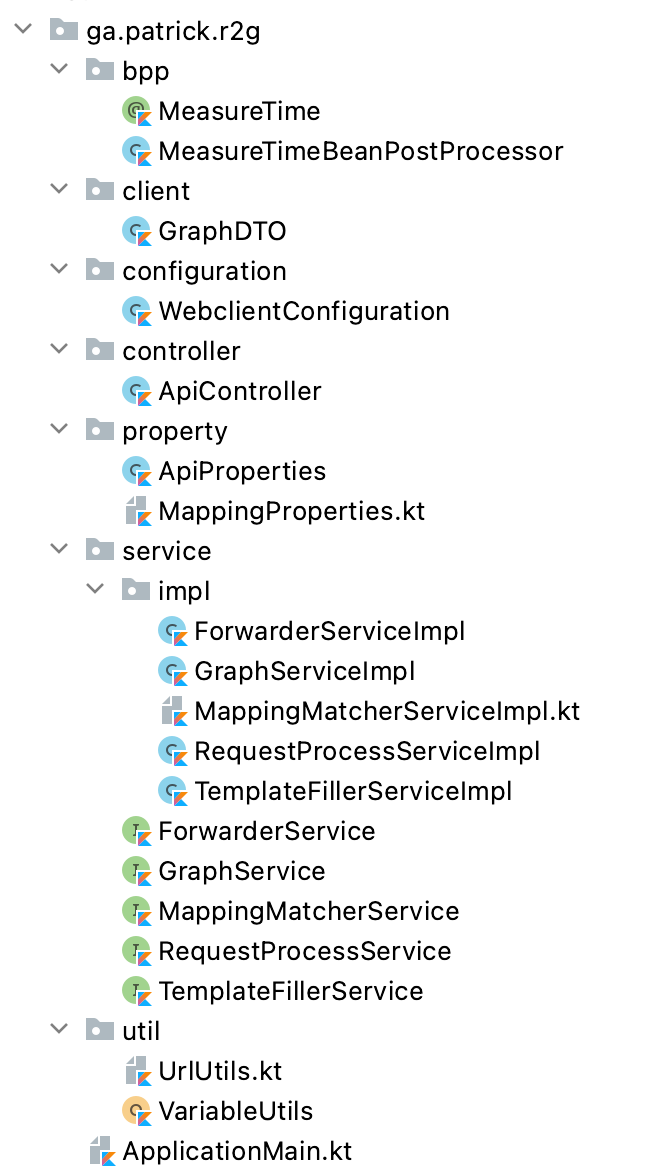
\includegraphics [scale=0.6] {my_folder/images/ch3-classes}
	\caption{Дерево пакетов модуля main}
	\label{fig:ch3-classes}
\end{figure}

\subsection{Пакет controller}\label{subsec:package-controller}

Данный пакет традиционно включает в себя классы, ответственные за принятие запроса к сервису и отправку ответа.
Каждый класс содержит набор методов с указаниями о том, какие запросы данный метод обрабатывает, и какие данные требуются для его работы.
Данные указания обычно даются в виде аннотаций.

Этот пакет имеет единственный класс ApiController, имеющий единственный метод endpoint.
Аннотация \texttt{@RequestMapping("/**")} указывает на то, что данный метод принимает запросы с любыми \texttt{path} и \texttt{method} (\texttt{GET}, \texttt{POST} и прочие).
Также, данный метод принимает в качестве аргумента объект \texttt{HttpServletRequest}, который содержит информацию о пришедшем запросе, такую как \texttt{path}, \texttt{method}, параметры \texttt{query}, тело запроса, словарь заголовков.
Таким образом, при получении любого запроса к данному веб-сервису информация об этом запросе будет передана в качестве аргументов при вызове этого метода.
Метод не имеет никакой логики, кроме вызова метода \texttt{processRequest} объекта \texttt{RequestProcessService}, который будет рассмотрен далее.

\subsection{Пакет service}\label{subsec:package-service}

Данный пакет включает в себя классы, ответственные за так называемую бизнес-логику.
В корне данного пакета находится ряд интерфейсов.
Интерфейсы используются в качестве контрактов для сервисов, которые планируется реализовать.
Подход, при котором сначала создаются интерфейсы, и только затем имплементации, широко используется при использовании Test Driven Development.
При использовании этого подхода котором прежде чем приступить к реализации продумывается внутренняя архитектура системы, создаются классы-интерфейсы, и для них пишутся тестовые сценарии, описывающие ожидаемое поведение системы.
Затем, классы, реализующие эти интерфейсы, помещяются в отдельных файлах, обычно в подпакетах с названием impl и именем, состоящим из названия интерфейса и постфикса Impl.
Также, данный подход позволяет создавать несколько реализаций для каждого интерфейса, позволяя подменять эти реализации перед запуском с помощью файла настроек, или даже в процессе работы программы.
Также, использование интерфейсов позволяет немного увеличить производительность и ускорить автоматизированное тестирование за счёт использования механизмов динамического проксирования JDK (Java Developer Kit), вместо технологии CGLIB\@.
Обе технологии используются для создания так называемых Proxy-объектов и Mock-объектов.

Proxy-объекты используются для неявного применения дополнительного поведения к какому-либо классу или методу, а также при использовании парадигмы АОП (Аспектно-ориентированное программирование).
Например, Proxy-объекты могут использоваться для кеширования ответа какого-либо метода, логирования аргументов и ответов методов, или для подсчёта времени выполнения метода.
В частности, последнее применение будет описано далее при обзоре аннотации \texttt{@MeasureTime} и класса \texttt{MeasureTimeBeanPostProcessor}.

Mock-объекты используются для эмуляции поведения какого-либо объекта в процессе проведения автоматизированного тестирования.
Например, какой-либо сервис в процессе своей работы осуществляет обращение к базе данных через некий бин.
Создание, наполнение и очистка базы данных для каждого теста являются значительными накладными расходами.
А в случае с сетевыми вызовами в большинстве случаев использование реального обращения к внешним сервисам (например, на тестовом или разработческом стенде) является либо невозможным, либо слишком медленным.
Кроме того, согласно методологии тестирования модули программы должны быть протестированы отдельно.
Поэтому для модульных (компонентных) тестов реализация зависимого бина подменяется Mock-объектом, для которого вручную задаётся определённое поведение.
Например, если бин получил в качестве аргумента строку \texttt{"a"}, то он должен будет ответить строкой \texttt{"b"}.
Применение Mock-объектов будет продемонстрировано в обзоре модуля \texttt{test}.

Технология CGLIB является более медленной, чем механизм динамического проксирования JDK, но механизм JDK работает за счёт реализации тех же интерфейсов, что и исходный класс.
Соответственно, для использования этого механизма JDK наш проксируемый/мокируемый класс должен реализовывать некий интерфейс.


Рассмотрим интерфейсы пакета service.
Согласно принципу Single Responsibility, каждый компонент имеет строгую зону ответственности.
Ответственность каждого из них описана ниже:

\begin{itemize}
	\item RequestProcessService -- является ключевым компонентом системы.
	Имеет единственный метод \texttt{processRequest}, который принимает объект входящего запроса \texttt{HttpServletRequest} и осуществляет отправку исходящего запроса к нужному сервису.
	В частности, этот метод получает соответствующий запросу маппинг, и в случае успеха формирует и отправляет запрос к соответствующему GraphQL-сервису.
	А в случае, если маппинг не был найден, перенаправляет запрос к некому серверу по умолчанию, указанному в настройках.

	\item MappingMatcherService -- используется для поиска маппинга, соответствующего входящему запросу.
	Он имеет единственный метод \texttt{findMapping}, который принимает объект запроса \texttt{HttpServletRequest}, находит и отдаёт соответствующий ему маппинг из настроек.

	\item TemplateFillerService – заполняет шаблон GraphQL-запроса параметрами, полученными из входящего запроса, в соответствии с маппингом.
	Компонент получает значения переменных для заполнения из URI, query parameters и тела запроса.

	\item GraphService – осуществляет отправку GraphQL-запроса.
	Имеет единственный метод send, принимающий URL запрашиваемого сервиса и объект GraphDTO, который будет отправлен в GraphQL-сервис.

	\item ForwarderService – перенаправляет запросы, для которых не нашлось маппинга, в Gateway API, указанный в настройках.
	Имеет единственный метод send, принимающий объект \texttt{HttpServletRequest}.
	Запрос передаётся с сохранением URI, headers, query parameters, тела и прочих параметров входящего запроса в исходном виде.

\end{itemize}

% Если маппинг не был найден, то он передаёт объект запроса в ForwarderService и возвращает ответ, полученный от Gateway API. Если маппинг был найден, то он использует TemplateFillerService для создания GraphQL-запроса, выполняет его с помощью GraphClient, который будет рассмотрен далее, и возвращает полученный ответ пользователю.


\subsection{Пакет util}\label{subsec:package-util}

Данный пакет включает в себя единственный класс VariableUtils, который содержит утилитарные методы для:

\begin{itemize}
	\item получения маски маппинга, которая будет использована для сравнения с пришедшим запросом;
	\item получения списка переменных, которые ожидается найти в пришедшем запросе;
	\item получения значения переменных из пришедшего запроса.
\end{itemize}

Для получения значений из тела запроса, представляющего из себя JSON, использована библиотека JsonPath.

\subsection{Пакет property}

Данный пакет содержит файл MappingProperties, содержащий следующие классы, по своей структуре повторяющие структуру маппингов, записанных в виде YAML-файла (например, application.yml):

\begin{itemize}
	\item MappingProperties -- корневой класс настроек.
	Он имеет в себе следующие поля:
		\subitem defaultEndpoint -- URL эндпоинта по умолчанию
		\subitem mappings -- список объектов типа Mapping, каждый из которых представляет собой описание правила для маппинга входящего запроса к исходящему, а также правило преобразования ответа.
		\subitem endpoints -- список доступных GraphQL-серверов.
		В этом списке указываются псевдонимы для URL этих серверов, чтобы избежать их многократного дублирования в маппингах.

	\item Mapping -- описание правила для маппинга входящего запроса к исходящему:
		\subitem path -- шаблон пути, который может содержать переменные;
		\subitem methods -- HTTP методы запроса;
		\subitem endpointName -- псевдоним GraphQL-сервера, на который нужно отправить запрос;
		\subitem template -- шаблон для запроса, представляющий собой GraphQL-запрос, возможно, содержащий в себе переменные, которые будут заполнены с помощью данных из входящего запроса.
		\subitem variables -- список объектов Variable -- описаний переменных, поддерживаемых GraphQL, которые используются в шаблоне, и значения для которых мы также получаем из входящего запроса.

	\item Endpoint -- объект, содержащий два поля:
		\subitem name -- псевдоним GraphQL-сервера;
		\subitem uri -- адрес этого сервера.

	\item VariableDefinition -- список переменных, которые следует отправить в составе GraphQL-запроса.
		\subitem name -- название переменной, используемой в GraphQL-запросе;
		\subitem source -- данные для получения значения этой переменной из входящего запроса;
		\subitem type -- тип данных переменной.
			Возможные значения содержатся в перечислении GraphVariableType.

	\item GraphVariableType -- набор возможных типов переменных.
		На данный момент поддерживаются строковые, целочисленные и дробные переменные.

\end{itemize}

\subsection{Пакет bpp}\label{subsec:package-bpp}

Данный пакет включает в себя класс \texttt{MeasureTimeBeanPostProcessor} и аннотацию \texttt{MeasureTime}.
Аннотация создана для замера скорости выполнения запроса, и должна быть поставлена на классе, скорость выполнения функций которого нас интересует.
Результаты использования этой аннотации будут более подробно рассмотрены в главе 4. % TODO ссылка

В данный момент эта аннотация стоит на классах \texttt{RequestProcessServiceImpl} и \texttt{GraphServiceImpl}. % TODO актуализировать
Соответственно, мы сможем засечь время выполнения функции \texttt{processRequest} и вычесть из него время выполнения фунции \texttt{send}, таким образом получив чистое время обработки запроса кодом приложения.

Класс \texttt{MeasureTimeBeanPostProcessor} отвечает за имплементацию логики засекания времени выполнения функций для классов, над которыми установлена аннотация \texttt{MeasureTime}.
Он является имплементацией \texttt{BeanPostProcessor}, которые в Spring Framework нужны для донастройки созданных бинов на разных этапах инициализации приложения.

Функция \texttt{postProcessBeforeInitialization} выполняется первой, и объект, который передаётся в качестве аргумента к этой фунции, является оригинальным бином (а не Proxy-объектом).
Вторым аргументом фунции является название (уникальный идентификатор) бина.
С помощью него мы сможем найти оригинальное описание класса, из которого был создан оригинальный бин.
Записываем название бина и информацию о его типе в словарь.

Функция \texttt{postProcessBeforeInitialization} выполняется второй.
Объект, получаемый в качестве аргумента, уже необязательно является оригинальным бином, а может являться Proxy-объектом, созданным другим \texttt{BeanPostProcessor}.
В свою очередь, Proxy-объекты могут не содержать всю нужную информацию, в частности, информацию об аннотациях, установленных над классом, его методами и полями.
Получаем информацию об оригинальном классе из словаря по имени бина.
Чтобы замерить время выполнения метода, создадим Proxy-объект, и зададим поведение для каждого метода.
При вызове каждого метода будем получать текущее системное время в миллисекундах, затем выполнять оригинальный метод проксируемого объекта, и после этого снова получать текущее системное время.
Вычтя из второго первое, получим время выполнения метода.
Запишем результат выполнения в словарь для последующей обработки, и также выведем в стандартный вывод (консоль).

\subsection{Модуль test}\label{subsec:module-test}

На \firef{fig:ch3-tests} изображено дерево пакетов модуля tests, содержащего исходные коды тестов, использующихся для автоматизированной проверки работоспособности приложения в целом, а также его компонентов по отдельности.

\begin{figure}[ht!]
	\center
	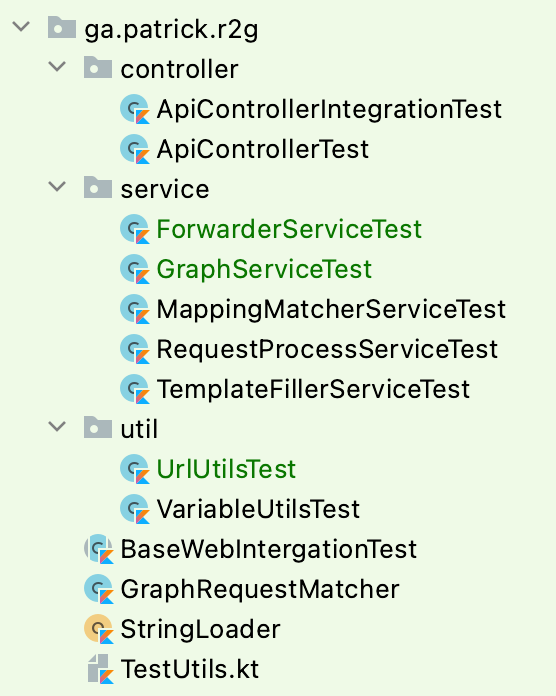
\includegraphics [scale=0.6] {my_folder/images/ch3-tests}
	\caption{Дерево пакетов модуля test}
	\label{fig:ch3-tests}
\end{figure}

% Рассмотрим тестовые классы более подробно: % ещё выше обещал рассказать про Mock'и

%\begin{itemize}

Данный модуль содержит в себе юнит-тесты для проверки работы ряда компоне, а также несколько интеграционных сервисов, проверяющих работоспособность системы вцелом.

Интеграционные тесты утилизируют тестовые данные, подготовленные ранее %в разделе 2.3
, причём вместо вызова внешних систем реализуются заглушки с помощью технологии WireMock, позволяющей указать ожидаемый запрос и соответствующий ему ответ.


\section{Выводы} \label{sec:ch3-conclusion}

В данной главе были поставлены требования к реализации системы, сформулированные на основании спецификации, описанной в теоретической части работы.
Были перечислены использованные технологии и представлены причины их выбора, и затем был приведён обзор исходного кода и разобраны некоторые примечательные детали реализации.
           	 % Глава 3
%! suppress = Unicode
\chapter{ТЕСТИРОВАНИЕ РЕАЛИЗАЦИИ} \label{ch4}

\textbf{Хорошим стилем является наличие введения к главе, которое \textit{начинается непосредственно после названия главы, без оформления в виде отдельного параграфа}.}

\section{Данные для тестирования реализации}\label{sec:testing-data}

Для тестирования сервиса R2G планируется использовать публичные GraphQL-сервисы.
В частности, сервис FakeQL позволяет создать GraphQL-сервис на основании данных в виде JSON. Для этого используем JSON, представленный в приложении 5.
Данный JSON загружается на сайт FakeQL, после чего мы получаем URL эндпоинта, к которому можно отправлять GraphQL-запросы.
Схема получившегося сервиса была продемонстрирована ранее (см. приложение 1).

В приложении 6 продемонстрирован пример маппинга.
для получения списка счетов в валюте из query parameter, для пользователя с идентификатором, переданным в URI. В приложении 7 представлен пример запроса, который соответствует указанному маппингу, а также GraphQL-запрос, который должен быть отправлен в GraphQL-сервер при получении такого запроса.

\section{Название параграфа} \label{ch4:sec1}

Для проверки работоспособности прототипа были использованы тестовые данные, подготовленные в разделе 2.3. Проверяются следующие сценарии:

\begin{itemize}
	\item Для запроса существует маппинг, не содержащий переменных.
	Система отправляет GraphQL-сервису шаблон из маппинга в неизменном виде и возвращает пользователю ответ.

	\item Для запроса существует маппинг, содержащий несколько переменных.
	Система заполняет шаблон этими переменными и отправляет результат GraphQL-сервису, возвращает пользователю ответ.

    \item Для запроса не существует маппинг.
	Запрос в неизменном виде перенаправляется по адресу Gateway API, указанному в настройках.
	В данном случае использовался сервис Postman Echo, возвращающий body и headers запроса в качестве ответа.
	Ответ этого сервиса возвращается пользователю.
\end{itemize}

Все сценарии были успешно проверены, в результате чего прототип считается работоспособным и будет использован для реализации целевой системы.


\section{Выводы} \label{ch4:conclusion}

Текст выводов по главе \thechapter.
           	 % Глава 3
\ContinueChapterEnd % завершить размещение глав <<подряд>>
%% Завершение основной части

%! suppress = Unicode
\chapter*{Заключение} \label{ch-conclusion}
\addcontentsline{toc}{chapter}{Заключение}	% в оглавление 

В процессе выполнения научно-исследовательской работы были изучены принципы технологий REST и GraphQL, определены их преимущества и недостатки, произведено сравнение между собой.
Смоделирован процесс миграции между данными технологиями и определены проблемы, возникающие при этом.

На основании полученных данных сформулированы принципы, лежащие в основе системы, которая должна стать альтернативой использованию каждой из указанных технологий в отдельности, а также упростить осуществлении миграции.

Для описанной системы определены её предполагаемые преимущества и недостатки, на основании чего принято решение о целесообразности реализации данной системы в процессе выполнения выпускной квалификационной работы.
Для этого было сформулировано техническое задание, включающее в себя требования к готовой системе, а также подготовлены тестовые данные, которые будут быть использованы для проверки работоспособности готовой системы.

По основным требованиям, сформулированным ранее, был реализован веб-сервис.
Для разработанного веб-сервиса была проведено функциональное тестирование на тестовых данных, а также произведена оценка его производительности. % TODO нагрузочное тестирование
На основании функционального тестирование было сделано заключение о жизнеспособности данного сервиса и данного подхода.
И на основании оценки производительности были предложены возможные способы улучшения скорости работы сервиса.

% песпективы внедрения
        	 % Заключение

%% Наличие следующих перечней не исключает расшифровку сокращения и условного обозначения при первом упоминании в тексте!
\chapter*{Список сокращений и условных обозначений}             % Заголовок
\addcontentsline{toc}{chapter}{Список сокращений и условных обозначений}  % Добавляем его в оглавление
\noindent
\addtocounter{table}{-1}% Нужно откатить на единицу счетчик номеров таблиц, так как следующая таблица сделана для удобства представления информации по ГОСТ
%\begin{longtabu} to \dimexpr \textwidth-5\tabcolsep {r X}
\begin{longtabu} to \textwidth {r X} % Таблицу не прорисовываем!
% Жирное начертание для математических символов может иметь
% дополнительный смысл, поэтому они приводятся как в тексте
% диссертации
\textbf{DOI} & Digital Object Identifier. \\
%$\begin{rcases}
%a_n\\
%b_n
%\end{rcases}$  & 
%\begin{minipage}{\linewidth}
%Коэффициенты разложения Ми в дальнем поле, соответствующие
%электрическим и магнитным мультиполям.
%\end{minipage}
%\\
%${\boldsymbol{\hat{\mathrm e}}}$ & Единичный вектор. \\
%$E_0$ & Амплитуда падающего поля.\\
%$\begin{rcases}
%a_n\\
%b_n
%\end{rcases}$  & 
%Коэффициенты разложения Ми в дальнем поле соответствующие
%электрическим и магнитным мультиполям ещё раз, но без окружения
%minipage нет вертикального выравнивания по центру.
%\\
%$j$ & Тип функции Бесселя.\\
%$k$ & Волновой вектор падающей волны.\\
%
%$\begin{rcases}
%a_n\\
%b_n
%\end{rcases}$  & 
%\begin{minipage}{\linewidth}
%\vspace{0.7em}
%Коэффициенты разложения Ми в дальнем поле соответствующие
%электрическим и магнитным мультиполям, теперь окружение minipage есть
%и добавленно много текста, так что описание группы условных
%обозначений значительно превысило высоту этой группы... Для отбивки
%пришлось добавить дополнительные отступы.
%\vspace{0.5em}
%\end{minipage}
%\\
%$L$ & Общее число слоёв.\\
%$l$ & Номер слоя внутри стратифицированной сферы.\\
%$\lambda$ & Длина волны электромагнитного излучения
%в вакууме.\\
%$n$ & Порядок мультиполя.\\
%$\begin{rcases}
%{\mathbf{N}}_{e1n}^{(j)}&{\mathbf{N}}_{o1n}^{(j)}\\
%{\mathbf{M}_{o1n}^{(j)}}&{\mathbf{M}_{e1n}^{(j)}}
%\end{rcases}$  & Сферические векторные гармоники.\\
%$\mu$  & Магнитная проницаемость в вакууме.\\
%$r,\theta,\phi$ & Полярные координаты.\\
%$\omega$ & Частота падающей волны.\\
%
%  \textbf{BEM} & Boundary element method, метод граничных элементов.\\
%  \textbf{CST MWS} & Computer Simulation Technology Microwave Studio.
\end{longtabu}
		         % Необязательная рубрика! Список сокращений и условных обозначений

%! suppress = Unicode
\chapter*{Словарь терминов}             % Заголовок
\addcontentsline{toc}{chapter}{Словарь терминов}  % Добавляем его в оглавление

\textbf{REST} --- архитектурный стиль построения взаимодействия между клиентом и сервисом.

\textbf{SOAP} --- протокол удалённого вызова процедур, передачи сообщений между системами в формате XML\@.

\textbf{GraphQL} --- язык запросов к серверу, использующий строгий синтаксис и схемы данных.

\textbf{Фронтенд (frontend)} --- клиентская часть системы, с которой напрямую осуществляет взаимодействие конечный пользователь.
Им может являться например мобильное, десктопное или веб-приложение.

\textbf{Бэкенд (backend)} --- серверная часть системы, обычно представляет собой набор сервисов.

\textbf{Сервис} --- серверное приложение, обрабатывающее запросы клиента.

\textbf{Эндпоинт (endpoint)} --- одна из, или единственная точка входа для запросов к сервису.

\textbf{Маппинг (mapping)} --- описание соответствия между двумя сущностями.

\textbf{Бин (bean)} --- объект, который управляется по принципу инверсии контроля (Inversion of Control) неким IoC-контейнером.
В данной работе роль IoC-контейнера выполняет Spring Framework.
    		 % Необязательная рубрика! Словарь терминов
% По порядку после Списка сокращений и условных обозначений, если есть.	


%%% Не мянять - Do not modify
%%
%%
\clearpage                                  % В том числе гарантирует, что список литературы в оглавлении будет с правильным номером страницы
%\hypersetup{ urlcolor=black }               % Ссылки делаем чёрными
%\providecommand*{\BibDash}{}                % В стилях ugost2008 отключаем использование тире как разделителя 
\urlstyle{rm}                               % ссылки URL обычным шрифтом
\ifdefmacro{\microtypesetup}{\microtypesetup{protrusion=false}}{} % не рекомендуется применять пакет микротипографики к автоматически генерируемому списку литературы
%\newcommand{\fullbibtitle}{Список литературы} % (ГОСТ Р 7.0.11-2011, 4)
%\insertbibliofull  
%\noindent
%\begin{group}
\chapter*{Список использованных источников}	
\label{references}
\addcontentsline{toc}{chapter}{Список использованных источников}    % в оглавление
\printbibliography[env=SSTfirst]      % Подключаем Bib-базы
%\ifdefmacro{\microtypesetup}{\microtypesetup{protrusion=true}}{}
%\urlstyle{tt}                               % возвращаем установки шрифта ссылок URL
%\hypersetup{ urlcolor={urlcolor} }          % Восстанавливаем цвет ссылок



%\urlstyle{rm}                               % ссылки URL о\dfrac{num}{den}бычным шрифтом
%\ifdefmacro{\microtypesetup}{\microtypesetup{protrusion=false}}{} % не рекомендуется применять пакет микротипографики к автоматически генерируемому списку литературы
%\insertbibliofull                           % Подключаем Bib-базы
%\ifdefmacro{\microtypesetup}{\microtypesetup{protrusion=true}}{}
%\urlstyle{tt}                               % возвращаем установки шрифта ссылок URL
		     % Список литературы

% Здесь можно поместить список иллюстративного материала

\appendix % не редактировать / keep unmodified


\chapter{Исходные коды приложения}\label{appendix-listings}
%\addcontentsline{toc}{chapter}{Second call for chapters to participate in the book Machine learning in analysis of biomedical and socio-economic data}  % Добавляем его в оглавление


\lstinputlisting{src/main/kotlin/ga/patrick/r2g/ApplicationMain.kt}

\lstinputlisting{src/main/kotlin/ga/patrick/r2g/bpp/MeasureTime.kt}
\lstinputlisting{src/main/kotlin/ga/patrick/r2g/bpp/MeasureTimeBeanPostProcessor.kt}

\lstinputlisting{src/main/kotlin/ga/patrick/r2g/client/GraphDTO.kt}

\lstinputlisting{src/main/kotlin/ga/patrick/r2g/configuration/WebClientConfiguration.kt}

\lstinputlisting{src/main/kotlin/ga/patrick/r2g/controller/ApiController.kt}

\lstinputlisting{src/main/kotlin/ga/patrick/r2g/property/ApiProperties.kt}
\lstinputlisting{src/main/kotlin/ga/patrick/r2g/property/MappingProperties.kt}

\lstinputlisting{src/main/kotlin/ga/patrick/r2g/service/ForwarderService.kt}
\lstinputlisting{src/main/kotlin/ga/patrick/r2g/service/impl/ForwarderServiceImpl.kt}
\lstinputlisting{src/main/kotlin/ga/patrick/r2g/service/GraphService.kt}
\lstinputlisting{src/main/kotlin/ga/patrick/r2g/service/impl/GraphServiceImpl.kt}
\lstinputlisting{src/main/kotlin/ga/patrick/r2g/service/MappingMatcherService.kt}
\lstinputlisting{src/main/kotlin/ga/patrick/r2g/service/impl/MappingMatcherServiceImpl.kt}
\lstinputlisting{src/main/kotlin/ga/patrick/r2g/service/RequestProcessService.kt}
\lstinputlisting{src/main/kotlin/ga/patrick/r2g/service/impl/RequestProcessServiceImpl.kt}
\lstinputlisting{src/main/kotlin/ga/patrick/r2g/service/TemplateFillerService.kt}
\lstinputlisting{src/main/kotlin/ga/patrick/r2g/service/impl/TemplateFillerServiceImpl.kt}

\lstinputlisting{src/main/kotlin/ga/patrick/r2g/util/UrlUtils.kt}
\lstinputlisting{src/main/kotlin/ga/patrick/r2g/util/VariableUtils.kt}

% TODO тестовые классы


\NewPage % начать новое приложение с новой страницы 			     % Приложение 1

%\chapter{Некоторые дополнительные примеры}\label{appendix-extra-examples}						    %

Приложение 2
			 	 % Приложение 2


\end{document} % конец документа


%%% Удачной защиты ВКР! - Good luck on the thesis defense!
%%
%%% Поддержать проект
%%
%% Запросы на добавление / изменение просим писать на следующей странице:
%% https://github.com/ParkhomenkoV/SPbPU-student-thesis-template/issues
%%
%% Список пожеланий в файле шаблона <<TO-DO-list.tex>>
%%
%% Благодарности просим указывать в виде 
%%
%% 1. Добавление <<Звезды>> проекту https://github.com/ParkhomenkoV/SPbPU-student-thesis-template/stargazers
%%
%% 2. Добавления <<Сердечка>> и репоста проекта в социальных сетях:
%%		https://vk.com/latex_polytech 
%%		https://www.fb.com/groups/latex.polytech
%%

%%% Support project
%%
%% Requests on adding / modifications is better to be publishen on the following web-page:
%% https://github.com/ParkhomenkoV/SPbPU-student-thesis-template/issues
%%
%% Wishlist is in the template's file called <<TO-DO-list.tex>>
%%
%% Acknowledgements are better to be done in the form of 
%%
%% 1. Adding <<Star>> to the project https://github.com/ParkhomenkoV/SPbPU-student-thesis-template/stargazers
%%
%% 2. Adding <<Likes>> and Project repost in the social networks:
%%		https://vk.com/latex_polytech 
%%		https://www.fb.com/groups/latex.polytech
%% 

% Check list при передаче ВКР:
% - Количество страниц в Задании 2. Если нет, то комментирование последней строки в my_task.tex
% - Зачистка всех вспомогательных файлов (Clear auxilary files) и компиляция ВКР не менее 3х раз